\documentclass[11pt]{article}
\usepackage[T1]{fontenc}
\usepackage{lmodern}
\usepackage[margin=1.05in]{geometry}
\usepackage{amsmath,amssymb,amsthm,mathtools}
\usepackage{microtype}
\usepackage{booktabs,array}
\usepackage{tikz}
\usetikzlibrary{arrows.meta,positioning,calc,fit,backgrounds}
\usepackage{xcolor}
\usepackage[hidelinks]{hyperref}
\hypersetup{pdftitle={Pointwise convergence of fourfold ergodic averages for mixing transformations},pdfauthor={OpenAI}}
\numberwithin{equation}{section}
\newtheorem{theorem}{Theorem}[section]
\newtheorem{proposition}[theorem]{Proposition}
\newtheorem{lemma}[theorem]{Lemma}
\newtheorem{corollary}[theorem]{Corollary}
\theoremstyle{definition}
\newtheorem{definition}[theorem]{Definition}
\theoremstyle{remark}
\newtheorem{remark}[theorem]{Remark}
\newcommand{\R}{\mathbb R}
\newcommand{\C}{\mathbb C}
\newcommand{\Z}{\mathbb Z}
\newcommand{\N}{\mathbb N}
\newcommand{\E}{\mathbb E}
\newcommand{\Prob}{\mathbb P}
\newcommand{\1}{\mathbf 1}
\newcommand{\dd}{\,d}
\newcommand{\norm}[1]{\lVert#1\rVert}
\newcommand{\abs}[1]{\lvert#1\rvert}
\newcommand{\ip}[2]{\langle#1,#2\rangle}
\newcommand{\CE}[2]{\E[#1\mid #2]}
\DeclareMathOperator{\Span}{span}
\DeclareMathOperator{\supp}{supp}
\DeclareMathOperator{\tr}{tr}
\DeclareMathOperator{\rank}{rank}
\DeclareMathOperator{\diag}{diag}
\DeclareMathOperator{\dist}{dist}
\setlength{\emergencystretch}{2em}
\title{Pointwise convergence of fourfold ergodic averages\newline for mixing transformations}
\author{OpenAI}
\date{October 4, 2026}
\begin{document}
\maketitle
\begin{abstract}
We prove that fourfold ergodic averages along the times $n,2n,3n,4n$
converge almost everywhere to the product of the integrals for every
invertible, bimeasurable, mixing probability-preserving transformation
and every fixed choice of bounded measurable inputs. Convergence holds
along all positive integer averaging lengths. No quantitative mixing
rate is assumed, and the probability space need not be standard.
\end{abstract}
\section{Introduction}\label{sec:introduction}

Let $(X,\mathcal F,\mu,T)$ be an invertible probability-preserving system.
For bounded measurable functions $f_1,\ldots,f_d$, the multiple ergodic
averages are
\[
A_N(f_1,\ldots,f_d)(x)
=\frac1N\sum_{n=1}^N\prod_{j=1}^d f_j(T^{jn}x).
\]
The general pointwise question asks whether these averages converge
almost everywhere for every finite $d$ on every invertible
probability-preserving system. Here we treat four functions under
the mixing hypothesis. We say that $T$ is mixing if
\begin{equation}\label{eq:mixing}
 \mu(A\cap T^{-n}B)\longrightarrow\mu(A)\mu(B)
 \qquad (|n|\longrightarrow\infty)
\end{equation}
for every $A,B\in\mathcal F$. The functions are fixed throughout each
convergence assertion. No rate in \eqref{eq:mixing} is assumed.

\begin{theorem}\label{thm:main}
Let $(X,\mathcal F,\mu)$ be a probability space and let $T:X\to X$
be invertible, bimeasurable, measure preserving, and mixing in the sense
of \eqref{eq:mixing}. For every $f_1,f_2,f_3,f_4\in L^\infty(\mu)$,
\[
 \frac1N\sum_{n=1}^N
 f_1(T^nx)f_2(T^{2n}x)f_3(T^{3n}x)f_4(T^{4n}x)
 \longrightarrow \prod_{j=1}^4\int_X f_j\dd\mu
\]
for $\mu$-almost every $x$, along all positive integers $N$.
The original probability space need not be standard.
\end{theorem}

\subsection*{Context and inputs}

Birkhoff's pointwise ergodic theorem treats a single observation along
an orbit \cite{Birkhoff}. Furstenberg's ergodic proof of Szemer\'edi's
theorem made products at arithmetic-progression times a central object
of study \cite{Furstenberg}. For weakly mixing transformations, these
averages converge in $L^2$ to the product of the integrals. For arbitrary
transformations, Host and Kra established norm convergence of every
finite consecutive length using nilpotent characteristic factors
\cite[Theorem~1.1]{HostKra}; Ziegler independently developed universal
characteristic factors and another proof \cite{Ziegler}. Norm
convergence alone does not control the exceptional lengths at an
individual point.

Bourgain proved pointwise convergence for two powers of one
transformation \cite{Bourgain}. Higher-order pointwise results include
$K$ systems \cite[Theorem~4.2]{DerrienLesigne}, weakly mixing systems
with suitable spectral restrictions \cite{Assani}, and weakly mixing
systems whose pairwise-independent finite self-joinings are all
product measures \cite{GutmanHuangShaoYe}. Huang, Shao and Ye proved
pointwise convergence of every finite consecutive length on ergodic
measure-distal systems \cite[Theorem~C]{HuangShaoYe}, extending the
distal investigation of Lesigne \cite{Lesigne}. Recent pointwise
theorems for polynomial iterates include the bilinear result of
Krause, Mirek and Tao \cite{KrauseMirekTao} and the distinct-degree
multilinear result of Kosz, Mirek, Peluse, Wan and Wright
\cite{KoszMirekPeluseWanWright}. Their degree hypotheses do not cover
the four linear iterates considered here. Kuca's survey \cite{Kuca}
gives a broader account of the norm and pointwise questions.

Theorem~\ref{thm:main} uses three companion results. The multiple-mixing
theorem of \cite[Theorem~1.1]{MixingCompanion} supplies mixing of every finite order
from \eqref{eq:mixing}. The analytic construction of
\cite{TripleCompanion}, based on the local estimates of
\cite{HilbertCompanion}, supplies an oscillation estimate for threefold
averages. Its oscillation assertion holds on arbitrary invertible
systems; mixing is used separately to identify limits. We need the
threefold estimate at each three-element subset of $\{1,2,3,4\}$.
Appendix~\ref{sec:lower-length} proves the required coefficient
adaptation and the resulting pointwise convergence lemma, including its
nonergodic formulation. The local analytic theorems themselves are cited
with their hypotheses and locations. Thus the contribution here is the
fourfold deduction from these specified inputs.

The structural part uses the Furstenberg--Zimmer theory of relatively
compact and relatively weakly mixing extensions. We record the
nonergodic and power-stability statements at their point of use in
Section~\ref{sec:structure}. The construction also uses extensions on
which certain conditional expectations cannot improve. Such energy
maximization belongs to the same general method as sated extensions
\cite{Austin}; the data being saturated here come from selected
four-coordinate laws.

\subsection*{The difficulty caused by selected lengths}

Suppose that the conclusion fails. After subtracting means, there are
four centred real functions and a positive-measure set of points at
which their averages remain positively separated from zero along
arbitrarily late lengths. We choose one such length $N_a(x)$ after
scale $2^a$. Averaging the configurations
\[
 (T^nx,T^{2n}x,T^{3n}x,T^{4n}x),\qquad 1\le n\le N_a(x),
\]
and passing to a limit preserves a nonzero correlation. A constant-roof
suspension makes these limit laws invariant under a flow and permits
the changes of speed needed later.

Selection is the main analytic obstruction. Conditioning on a length
chosen from the initial state can change the joint law of independent
auxiliary variables. Ordinary norm convergence, with no
rate, does not by itself bound all the resulting errors. We introduce
three groups of auxiliary spatial coordinates. Their joint law is a
product, and any two groups together are independent of the original
coordinate, after conditioning on the suspension phases. A length
event may change the full three-group law, but preserves the
two-group marginals. This is precisely the amount of independence used
in Section~\ref{sec:channels}. For a finite model of the distinction,
let $U,V,W$ be independent symmetric signs. Their product is independent
of each pair, but conditioning on $UVW=1$ constrains the triple.

The estimate making this possible is a finite-dimensional packing
statement proved in Section~\ref{sec:packing}. If two bounded families
of Hilbert-space vectors have small pairwise inner products outside a
graph of bounded degree, few of their tensor products can have large
projection onto a subspace of slowly growing dimension. A Gaussian
comparison and a trace-moment estimate give a quantitative form of
this assertion. Applied to the leading covariance subspace, it controls
the projected part of each selected average. The complementary part
has a square-summable error over the possible lengths. The estimate is
independent of the ambient Hilbert-space dimensions and requires no
quantitative mixing rate.

\subsection*{From a correlation to a contradiction}

Each auxiliary system carries both an original spatial coordinate and
the three groups of additional coordinates. We call such a system a
channel after specifying its exact independence conditions in
Definition~\ref{def:channel}. In its selected four-coordinate law,
consider nonzero correlations in which each slot uses either a
centred function of the original coordinate or a centred function of
the additional coordinates. Bounded functions of the distal parameters
are allowed as weights. The initial failure gives a correlation with
no additional-coordinate slots.

Choose a channel and a correlation maximizing the number of slots of
the second kind. Independence excludes four such slots. An iterated
array construction excludes three: products along different axes
through a fixed corner are orthogonal, but each has the same nonzero
correlation with the function at that corner. Bessel's inequality
rules this out. At most two slots can therefore be of the second kind.

The final construction increases that number. First enlarge the
channel until the conditional expectations needed by the argument
are stable under further extensions. Then regard one selected
four-coordinate law as a new system and select once more. The result
is a square of old states. Its distinguished row and column meet at
one corner; saturation supplies their exact conditional laws. A
reanchoring identity on the distal parameters shows that the row and
column correlation cannot vanish. Regrouping the other coordinates
therefore replaces one original-coordinate slot by an
additional-coordinate slot, contradicting maximality.

Sections~\ref{sec:structure} and~\ref{sec:selected} establish the
structural inputs and selected laws. The packing estimate and channel
preservation are proved in Sections~\ref{sec:packing}
and~\ref{sec:channels}. Section~\ref{sec:activation} carries out the
maximality argument and completes the proof. The coefficient-dependent
analytic work is collected in Appendix~\ref{sec:lower-length}.

\section{Convergence inputs and relative structure}
\label{sec:structure}

The auxiliary systems in the proof will be extensions and joinings of a
suspension of the original transformation.  They need not be ergodic.
We therefore formulate the structural facts in the nonergodic setting,
and distinguish the pointwise input for three functions from the norm
estimate available for any finite number of functions.

\subsection{Standard systems and the pointwise inputs}

Put $I=\{1,2,3,4\}$.  It suffices to prove
Theorem~\ref{thm:main} on a standard probability space.  Indeed, for a
given tuple of bounded functions, the map recording all their integer
translates takes values in a countable product of compact scalar discs.
The pushforward measure and the shift give a standard factor, the
functions descend to its coordinate functions, and mixing passes to
this factor.  Almost-sure convergence there pulls back to the original
space.  We henceforth write $(X,\mu,T)$ for this standard mixing system.
All factors and conditional expectations are understood modulo null
sets; probability spaces may be completed.

We use \cite[Theorem~1.1]{MixingCompanion} in the following
form.  For every fixed finite family $g_1,\ldots,g_s\in L^\infty(\mu)$,
\begin{equation}\label{eq:all-orders-input}
 \int_X\prod_{j=1}^s g_j(T^{n_j}x)\,\dd\mu(x)
 \longrightarrow \prod_{j=1}^s\int_Xg_j\,\dd\mu
 \quad\text{if}\quad \min_{j\ne l}|n_j-n_l|\longrightarrow\infty.
\end{equation}
The bounded-function formulation follows from the set formulation by
simple-function approximation.  All uses of this input involve fixed
functions; no rate of mixing is assumed.

The other companion input will be used on systems without mixing.
Its coefficient dependence is important, so we isolate its exact scope.

\begin{lemma}[Lower-length convergence]\label{lem:lower-length}
Let $(Y,m,R)$ be an invertible probability-preserving transformation on
a standard probability space.  If $\varnothing\ne J\subsetneq I$ and
$g_i\in L^\infty(m)$ for $i\in J$, then
\[
 \frac1N\sum_{n=1}^N\prod_{i\in J}g_i(R^{in}y)
\]
converges for $m$-almost every $y$.
\end{lemma}

The proof, including the changes of coefficients in the analytic
estimates of \cite{TripleCompanion,HilbertCompanion}, is given in
Appendix~\ref{sec:lower-length}.  Neither ergodicity nor mixing is an
assumption of Lemma~\ref{lem:lower-length}.

\subsection{Distal factors and relatively weakly mixing extensions}

Let $(Y,m,R)$ be a standard probability-preserving system, and let
$B$ be a factor.  We use the conditional-correlation characterization
of \emph{relative weak mixing}: for bounded $f,g$, with
$\E[f\mid B]=0$,
\begin{equation}\label{eq:rwm-correlations}
 \frac1H\sum_{h=1}^H
 \bigl\|\E[\overline f\,(g\circ R^h)\mid B]\bigr\|_2^2
 \longrightarrow0.
\end{equation}
For $F_1,\ldots,F_r\in L^2(m)$, the associated finitely generated
$L^\infty(B)$-module is
\[
 \left\{\sum_{j=1}^r a_j F_j:a_j\in L^\infty(B)\right\}.
\]
It is invariant if composition with $R$ and with $R^{-1}$ preserves
this space.  An extension is \emph{relatively compact} if its $L^2$
space is generated by these invariant modules.
The individual modules need not be closed in $L^2$; closure is taken
after their union is spanned.  This is the compact-module
characterization in its corrected form
\cite[Theorem~4.1]{Jamneshan}\cite[Theorem~2.5]{JamneshanCorrigendum}.
A
\emph{relatively distal} extension is a tower of relatively compact
extensions and inverse limits.  Distality without a specified base
means distality over the trivial factor.  These definitions include
nonergodic systems; in particular an identity action is compact.

\begin{proposition}[Relative structure]\label{prop:structure}
The following statements hold for standard probability-preserving
systems.
\begin{enumerate}
\item There is a maximal measure-distal factor $W_Y$.  It contains the
invariant factor, and $Y\to W_Y$ is relatively weakly mixing.  A distal
factor pulls back into the maximal distal factor of any extension.
Every measure-preserving automorphism commuting with $R$ preserves
$W_Y$.
\item Factors and joinings of distal systems are distal.  A distal
system is relatively distal over each of its factors.  For every
nonzero integer $q$, $R$ is distal if and only if $R^q$ is distal.
\item Relative weak mixing passes to nonzero integer powers and to
conditionally independent base change.  More generally, the product
of relatively weakly mixing fibre laws over any invariant joining of
their base laws is relatively weakly mixing over that joining.
\item A relatively weakly mixing extension and a relatively distal
extension of the same base are relatively disjoint: the only invariant
joining which identifies their base coordinates is the relatively
independent joining.
\item If $R$ is distal, then, for every $d\ge1$ and bounded
$g_1,\ldots,g_d$, the averages
\[
 \frac1N\sum_{n=1}^N\prod_{i=1}^d g_i(R^{in}y)
\]
converge almost surely.
\end{enumerate}
If $(S_Y^t)_{t\in\R}$ is a probability-preserving flow, the maximal
distal factor $W_Y$ of $S_Y^1$ is a flow factor.  Its action at every
nonzero rational time is distal.
\end{proposition}

\begin{proof}
The existence assertion and the relatively weakly mixing extension
are the Furstenberg--Zimmer structure theorem
\cite{Furstenberg,Zimmer}; its nonergodic probability-algebra formulation
is given in \cite[Theorems~1.1 and~1.2]{Jamneshan}.
We recall the consequences needed here, with particular attention to
changes of base and of time.

At a compact stage, an invariant finitely generated module remains such a
module after the base is enlarged.  One may use bounded generators:
for a vector of generators transforming by unitary matrices over the
base, truncate by its invariant pointwise length.  Products of bounded
generators lie in finitely generated tensor modules.  Consequently the join
of compact stages is compact over the joined base, and the same
assertion for distal towers follows by passing to closures at limit
stages.  This proves closure under joinings and the assertion about
enlarging the base to any factor of a distal system.  It also shows
that distal factors of a system lie in its maximal distal factor.
Applying this observation to an automorphism commuting with $R$, and
then to its inverse, shows that it preserves $W_Y$.  The invariant
factor is compact and therefore belongs to $W_Y$.

Compact modules for $R$ are compact modules for $R^q$, so distality
passes to powers.  Conversely, suppose $q>0$ and $R^q$ is distal.
Its canonical compact tower is preserved by $R$, which commutes with
$R^q$.  At each successor stage replace an $R^q$-invariant finitely
generated module by the sum of its first $q$ translates under $R$.
This is a finitely generated $R$-invariant module over the same base.
The resulting tower
proves distality for $R$.  Negative powers give the same conclusion
by inversion.

For relative weak mixing, the nonnegative summands in
\eqref{eq:rwm-correlations} show that restriction to multiples of a
fixed positive integer still has Ces\`aro limit zero.  Invariance and
complex conjugation handle negative powers.  To verify the assertion
about joined bases, let $Y_j\to B_j$ be the extensions and let $\sigma$
be an invariant joining of the base measures.  On the resulting space
give the fibres the law
\[
 \int\bigotimes_j m_j(\dd y_j\mid b_j)\,\dd\sigma((b_j)_j).
\]
For bounded tensor tests, their conditional correlation over the full
base has the form
\begin{equation}\label{eq:product-rwm-correlation}
 a(b)\,c(S_B^h b)
 \prod_j\E[\overline{f_j}\,(g_j\circ R_j^h)\mid B_j](b_j).
\end{equation}
If one $f_j$ is conditionally centred, the squared $L^2(\sigma)$ norm
is bounded by a constant times the squared norm of that factor in
$L^2(B_j)$.  Here only the $j$th marginal of $\sigma$ is used.
Its Ces\`aro mean tends to zero.  Subtracting the conditional
expectation of a tensor and telescoping shows that such centred
tensors span a dense subspace of the orthocomplement of the full
base.  Bounded approximation now proves the claim.  The same
calculation with an arbitrary extra base coordinate proves stability
under conditionally independent base change.

For relative disjointness we argue with conditional modules.  The
absolute weak-mixing disjointness principle goes back to
Furstenberg~\cite[Part~I, Section~7]{FurstenbergDisjointness}.
First take a compact extension of the base.  A joining defines a
base-linear, time-intertwining conditional
expectation operator from its $L^2$ space to the relatively weakly
mixing side.  It takes each finitely generated invariant module into
another such module.  Relative weak mixing says that the latter lies
in the base, so the joining is relatively independent.  Induct along
a distal tower: once independence has been proved at a stage, the
extension on the other side is the conditionally independent base
change of the original relatively weakly mixing extension.  The
preceding calculation allows the compact-stage argument to be
repeated.  Conditional expectations pass to the limit at limit
stages.  This proves relative disjointness without an ergodicity
assumption.  It also gives closure of distal systems under factors:
if $D$ is distal and $B$ is its factor, then $D$ is distal over the
pullback of $W_B$; relative disjointness of $D\to W_B$ and
$B\to W_B$ forces the latter extension to be trivial.

For the pointwise assertion, the ergodic case is
\cite[Theorem~C]{HuangShaoYe}, whose distality is measure-theoretic.
For a nonergodic distal system, start its compact tower with the
invariant factor and disintegrate over that factor.  The tower is
countable on a standard space: its genuinely increasing successor
stages give nonzero orthogonal differences in a separable $L^2$
space.  At each stage choose a countable generating algebra.  Approximate
each of its indicators by functions in the compact modules at a
successor stage, or in the preceding factors at a limit stage, with
summable squared $L^2$ errors.  Fubini makes these errors summable in
the conditional $L^2$ spaces on almost every ergodic component,
simultaneously for all the chosen approximations.  The restricted
generating algebras are dense for every component measure.  The
countably many identities expressing invariance of the chosen modules
also disintegrate.  Thus the successor stages remain compact and the
limit stages remain generated by their predecessors on a common
conull set of components.  Every intermediate factor has the same invariant
algebra, so each component tower consists of ergodic systems; its
compact extensions are isometric by the compact-extension structure
theorem.  Each component is thus an ergodic distal system.
The cited theorem applies to the given tuple on almost every
component, proving the assertion.

Finally, every flow time commutes with time one and therefore
preserves $W_Y$.  If $r=p/q\ne0$ is rational, the $q$th power of
its action on $W_Y$ is the distal action at integer time $p$.
The power assertion gives distality at time $r$.
\end{proof}

The following norm estimate explains why proper subaverages have a
particularly simple law over a distal factor.  Its proof uses relative
weak mixing alone.

\begin{lemma}[A relatively weakly mixing characteristic factor]
\label{lem:relative-norm}
Suppose $Y\to B$ is relatively weakly mixing for an invertible
transformation $R$.  If $a_1,\ldots,a_d$ are distinct nonzero integers
and $g_1,\ldots,g_d$ are bounded, then
\begin{equation}\label{eq:relative-norm}
 \left\|\frac1N\sum_{n=1}^N
 \left(\prod_{i=1}^d g_i\circ R^{a_i n}
 -\prod_{i=1}^d\E[g_i\mid B]\circ R^{a_i n}\right)\right\|_2
 \longrightarrow0.
\end{equation}
\end{lemma}

\begin{proof}
By telescoping and scaling, it suffices to consider functions bounded
by one, one of which, say $g_s$, has conditional mean zero.  We induct
on $d$, with the empty product as the initial case.  Set
$v_n=\prod_i g_i\circ R^{a_i n}$ and, for a fixed $h\ge1$, put
$F_{i,h}=\overline{g_i}(g_i\circ R^{a_i h})$.
Invariance gives
\[
 \langle v_n,v_{n+h}\rangle
 =\int F_{s,h}\prod_{i\ne s}
       F_{i,h}\circ R^{(a_i-a_s)n}\,\dd m.
\]
The other coefficients are distinct and nonzero.  The induction
hypothesis replaces their factors, in the average over $n$, by
their conditional expectations over $B$, with an error tending to
zero.  Those remaining factors are $B$-measurable and bounded by
one, so
\[
 \limsup_{N\to\infty}
 \left|\frac1N\sum_{n=1}^N\langle v_n,v_{n+h}\rangle\right|
 \le \|\E[F_{s,h}\mid B]\|_1.
\]
For $d=1$ the same inequality holds directly.  The Hilbert-space
van der Corput inequality bounds the squared norm of the averages
of $v_n$ by an absolute constant times
\[
 \frac1H+\frac1H\sum_{h=1}^H\|\E[F_{s,h}\mid B]\|_1
\]
in the limit superior as $N\to\infty$.  The second term tends to
zero by \eqref{eq:rwm-correlations} for $R^{a_s}$ and
Cauchy--Schwarz.  Letting $H\to\infty$ proves the induction.
\end{proof}

In particular, weak mixing of $T$ gives $L^2$ convergence to the
product of the means for all finite distinct nonzero linear powers
on $X$.  In a flow, with $B$ preserved by every time, the analogue of
\eqref{eq:relative-norm} for deterministic continuous-time averages
follows by writing $t=n+s$, $0\le s<1$.  Apply the lemma for each
fixed $s$ to $g_i\circ S_Y^{a_i s}$, and integrate the resulting
$L^2$ estimate in $s$.  Conditional expectation commutes with these
time shifts.  Bounded convergence and the final interval of length
less than one complete the passage to continuous time.

\section{Selected laws and their distal parameters}
\label{sec:selected}

A failure of pointwise convergence allows the averaging length to
depend on the initial state.  We encode this failure in a probability
law on four outputs.  The selection can change their joint law, but
the convergence results of Section~\ref{sec:structure} will determine
every proper marginal, even after all distal parameters are given.

\subsection{From failure to a sequence of selectors}

Let $C=X\times[0,1)$ have measure $m_C=\mu\otimes\dd u$ and the
roof-one suspension flow
\begin{equation}\label{eq:suspension}
 S_C^t(x,u)=\bigl(T^{\lfloor u+t\rfloor}x,\{u+t\}\bigr).
\end{equation}
Write $\xi:C\to X$ for its spatial coordinate and
$\upsilon:C\to\R/\Z$ for its phase.  The use of a flow will let
us normalize the action at any one of the four outputs.

\begin{proposition}[Selectors witnessing failure]\label{prop:selectors}
If Theorem~\ref{thm:main} fails, there are real functions
$f_i\in L^\infty(\mu)$ with $\|f_i\|_\infty\le1$ and
$\int f_i\,\dd\mu=0$, a finite set $F\subset[1,2]$, measurable
functions
\[
 N_a:C\longrightarrow\{c2^k:c\in F,\ k\ge a\},\qquad a\ge1,
\]
a continuous real function $\Psi$ on $(\R/\Z)^I$, and
$\epsilon_0>0$ such that, for all sufficiently large $a$,
\begin{equation}\label{eq:selected-positive}
 \int_C\frac1{N_a(z)}\int_0^{N_a(z)}
 \Psi\bigl((\upsilon(S_C^{it}z))_{i\in I}\bigr)
 \prod_{i\in I}f_i\bigl(\xi(S_C^{it}z)\bigr)
 \,\dd t\,\dd m_C(z)\ge\epsilon_0.
\end{equation}
The selectors may be chosen independent of the initial phase.
\end{proposition}

\begin{proof}
Expand each function in the failed assertion into its mean and its
centred part.  Lemma~\ref{lem:lower-length} and the $L^2$ conclusion
of Lemma~\ref{lem:relative-norm} show that every proper subaverage
converges almost surely to the product of its means.  Thus a
fourfold average of centred functions fails to converge to zero.
Expanding real and imaginary parts and scaling gives a real tuple
bounded by one with the same property.  Its averages
\[
 A_N(x)=\frac1N\sum_{n=1}^N\prod_{i\in I}f_i(T^{in}x)
\]
converge to zero in $L^2$.  After changing the sign of one function
if necessary, there are $\delta>0$ and a measurable set $E$ of
positive measure such that $A_N(x)>2\delta$ for arbitrarily large
$N$, for every $x\in E$.

For bounded summands, changing the averaging length from $N$ to $M$
changes the average by at most $2|N-M|/\max(N,M)$.  Choose a finite
grid $F\subset[1,2]$ fine enough that arbitrarily late inequalities
$A_N(x)>2\delta$ yield arbitrarily late lengths $L=c2^k$ satisfying
$A_{\lfloor L\rfloor}(x)>\delta$.  The rounding error tends to zero
uniformly as $k\to\infty$.  For $x\in E$, choose measurably, from a
fixed enumeration, one such length with $k\ge a$.  Set $N_a(x,u)$
equal to that choice.  For $x\notin E$, set $N_a(x,u)=2^a$, including
$1$ in $F$.  Countability of the available lengths gives measurable
selectors.

Choose nonnegative continuous functions $\alpha,\beta$ on $\R/\Z$,
not identically zero, with supports respectively in $(1/4,1/2)$ and
$(0,1/16)$.  Define
\[
 \Psi(v_1,v_2,v_3,v_4)
 =\alpha(2v_1-v_2)\,\beta(v_2-v_1).
\]
For output phases $v_i=u+it\pmod1$, this equals
$\alpha(u)\beta(\{t\})$.  On its support, writing $t=n+s$ with
$0\le s<1$ gives $0<u+is<1$ for every $i\in I$.
Consequently the spatial outputs in \eqref{eq:selected-positive}
are precisely $T^{in}x$.  If $b_\beta=\int_0^1\beta(s)\,\dd s$,
integration over complete unit intervals yields, uniformly in $x,u$
and $L\ge2$,
\begin{equation}\label{eq:phase-selector-comparison}
 \frac1L\int_0^L\Psi\bigl((u+it)_{i\in I}\bigr)
       \prod_i f_i\bigl(\xi(S_C^{it}(x,u))\bigr)\,\dd t
 =\alpha(u)b_\beta A_{\lfloor L\rfloor}(x)+O(L^{-1}).
\end{equation}
The shift from the indices $0,\ldots,\lfloor L\rfloor-1$ to
$1,\ldots,\lfloor L\rfloor$ costs another $O(L^{-1})$.

The integral of the right side over $E\times[0,1)$ is at least
$\delta\mu(E)b_\beta\int\alpha+o(1)$.  Over the complement of $E$
the selected length is deterministic, and $A_{2^a}\to0$ in $L^2$,
so its contribution tends to zero.  The constant in front of
$\mu(E)$ is positive.  Choosing $\epsilon_0$ smaller than its
product with $\delta\mu(E)$ proves the proposition.
\end{proof}

For the rest of the proof assume failure and fix the functions,
selectors and phase test of Proposition~\ref{prop:selectors}.
We use one fixed free ultrafilter $\mathcal U$ on the indices $a$.

\subsection{A functorial law on four outputs}

Consider a standard probability-preserving flow
$(Y,m_Y,S_Y^t)$ with an equivariant factor $\pi_Y:Y\to C$.
The selector on $Y$ is $N_a\circ\pi_Y$.  For bounded measurable
functions $G_i$ on $Y$, define the selected law by
\begin{equation}\label{eq:selected-law}
 \int_{Y^I}\prod_{i\in I}G_i(y_i)\,\dd\lambda_Y
 =\lim_{a\to\mathcal U}
 \int_Y\frac1{N_a(\pi_Yy)}
 \int_0^{N_a(\pi_Yy)}\prod_{i\in I}G_i(S_Y^{it}y)
 \,\dd t\,\dd m_Y(y).
\end{equation}
The existence of a countably additive law with this formula is part
of the next proposition.

Let $\omega_Y:Y\to W_Y$ be the maximal distal factor of time one,
write $\nu_Y=(\omega_Y)_*m_Y$, and disintegrate
$m_Y=\int m_{Y,w}\,\dd\nu_Y(w)$.  For a state
$(y_i)_{i\in I}$ of the selected law, put
$P_i=\omega_Y(y_i)$ and $P=(P_i)_{i\in I}$.

\begin{proposition}[Selected laws]\label{prop:selected}
Formula~\eqref{eq:selected-law} defines a probability measure
$\lambda_Y$ on $Y^I$ with the following properties.
\begin{enumerate}
\item Every marginal is $m_Y$, and $\lambda_Y$ is invariant under
$(y_i)_i\mapsto(S_Y^{it}y_i)_i$ for every $t\in\R$.
If $\theta:Y'\to Y$ is an extension over $C$, then
$(\theta^I)_*\lambda_{Y'}=\lambda_Y$.  These projections also hold
for countable inverse limits of extensions.
\item The law $\Lambda_Y$ of $P$ is its deterministic-length law:
for bounded $H_i$ on $W_Y$,
\begin{equation}\label{eq:ordinary-parameter-law}
 \int\prod_iH_i(w_i)\,\dd\Lambda_Y
 =\lim_{L\to\infty}\int_Y\frac1L\int_0^L
       \prod_i H_i(\omega_Y(S_Y^{it}y))\,\dd t\,\dd m_Y(y).
\end{equation}
\item For every proper subset $J\subsetneq I$, the conditional law
of $(y_i)_{i\in J}$ given the \emph{entire} parameter array $P$ is
\begin{equation}\label{eq:proper-fibres}
 \operatorname{Law}_{\lambda_Y}\bigl((y_i)_{i\in J}\mid P\bigr)
 =\bigotimes_{i\in J}m_{Y,P_i}.
\end{equation}
\end{enumerate}
In a countable inverse limit, functions pulled back from the selected
laws at finite stages are dense in the $L^2$ space of the limiting
selected law.
\end{proposition}

\begin{proof}
Denote the finite-$a$ law in the right side of
\eqref{eq:selected-law} by $\lambda_{Y,a}$.  For a single bounded
measurable function $G$, the ordinary pointwise ergodic theorem for
the flow gives, since $N_a\ge2^a$,
\[
 \frac1{N_a(\pi_Yy)}\int_0^{N_a(\pi_Yy)}G(S_Y^{it}y)\,\dd t
 \longrightarrow \E[G\mid\mathcal I_Y](y)
\]
almost surely, where $\mathcal I_Y$ is the invariant factor of the
flow.  Integrating proves convergence of each marginal against
every bounded measurable test to $m_Y$.  Ergodicity is unnecessary.

Realize $Y$ as a Borel subset of a compact metrizable space $K$.
The ultralimit of the integrals of continuous functions on $K^I$
is a positive functional of mass one, hence a probability measure.
Its marginals are $m_Y$, so it is concentrated on $Y^I$.
For bounded measurable slot functions, approximate each in
$L^1(m_Y)$ by continuous functions on $K$, with the same uniform
bound.  The error in a product test is bounded by the sum of the
errors in the individual marginal tests.  The preceding marginal
convergence makes this bound valid in the ultralimit as well as
under the limiting measure.  Letting the approximation errors tend
to zero proves \eqref{eq:selected-law} for all bounded slot tests.

Applying the product action at time $s$ shifts the inner integration
interval from $[0,N_a]$ to $[s,N_a+s]$.  For tests bounded by one the
error is at most $2|s|/2^a$.  This proves invariance.  Notice that
the selector is still evaluated at the same initial state; no
invariance of the selector is required.  Pulling back product tests
under an extension over $C$ leaves the selector unchanged and proves
functoriality.  A countable inverse limit is again a standard flow,
and the same formula gives its stated projections.  Its coordinate
$\sigma$-fields are generated by the stage coordinate factors;
finite products of their functions are dense, proving the last
assertion.  Strong continuity of the product flow in its new $L^2$
space follows first on tensors from the fixed marginal laws and
then by density.

We next determine the parameter and proper-slot laws.  The pointwise
theorem for the distal system $W_Y$ passes to continuous time as
follows.  Write $t=n+s$, $0\le s<1$.  For each fixed $s$ apply
Proposition~\ref{prop:structure}(5) to the shifted functions
$H_i\circ S_{W_Y}^{is}$.  Fubini and bounded convergence give
pointwise convergence after integrating $s$, while the final
incomplete unit interval contributes $O(L^{-1})$.  Thus the
continuous averages converge almost surely along all real lengths.
Their value at any selected length $N_a(\pi_Yy)$ has the same
limit.  Integration gives \eqref{eq:ordinary-parameter-law}.

For a proper subset $J$, apply precisely this time decomposition to
Lemma~\ref{lem:lower-length}, now on $Y$ itself.  Its selected
$J$-slot marginal is consequently the deterministic-length law.
The continuous-time version of Lemma~\ref{lem:relative-norm}, over
$W_Y$, replaces every slot test $G_i$ in that law by
$\E[G_i\mid W_Y]$.  We may also multiply each slot test by an
arbitrary bounded function of its parameter.  It follows that,
given the parameter subarray $(P_i)_{i\in J}$, this marginal has
the conditional product law $\bigotimes_{i\in J}m_{Y,P_i}$.

It remains to condition on the parameters outside $J$; marginal
conditional independence alone would not justify this step.
Under the time-one action with speeds $i$, the law just identified
is a relatively weakly mixing extension of its parameter subarray.
Indeed, each $Y\to W_Y$ is relatively weakly mixing for the
corresponding power, and Proposition~\ref{prop:structure}(3)
applies over the joining of the base laws.  The law of the full
parameter array is a joining of the distal systems
$(W_Y,S_{W_Y}^i)$.  It is therefore distal, and relatively distal
over the parameter subarray.  The joint law of the $J$ states and
all parameters is an invariant joining of these two extensions
over their common base.  Relative disjointness forces it to be
the relatively independent one.  This is exactly
\eqref{eq:proper-fibres}.
\end{proof}

For $b\in I$ define the normalized flow
\begin{equation}\label{eq:normalized-selected-flow}
 \mathsf M_b(Y)=
 \left(Y^I,\lambda_Y,
       (y_i)_i\longmapsto(S_Y^{it/b}y_i)_i\right).
\end{equation}
Its projection to slot $b$ is an equivariant extension of $Y$ and
therefore of $C$.  This permits the selected-law construction to be
iterated with the same selectors and the same ultrafilter.

\begin{lemma}[Distal parameters after normalization]
\label{lem:parameter-distal}
The full parameter array $(\omega_Y(y_i))_{i\in I}$ is a distal
factor of the time-one map of $\mathsf M_b(Y)$, and hence belongs
to its maximal distal factor.  The same assertion holds for the
arrays of original parameters in every finite iteration of
normalized selected flows.
\end{lemma}

\begin{proof}
In slot $i$ the action on the parameter is $S_{W_Y}^{i/b}$,
which is distal by Proposition~\ref{prop:structure}.  The full
array is a joining of these distal systems and is therefore distal.
At the next iteration the old distal factors pull into the new
maximal distal factors.  Induction proves the iterated assertion.
\end{proof}

Finally, the phase test in Proposition~\ref{prop:selectors} can be
approximated uniformly by finite sums of products of one-slot phase
functions.  Formula~\eqref{eq:selected-law} therefore applies to its
product with the four spatial tests.  In particular,
\begin{equation}\label{eq:initial-selected-witness}
 \int_{C^I}\Psi\bigl((\upsilon(z_i))_i\bigr)
       \prod_i f_i(\xi(z_i))\,\dd\lambda_C\ge\epsilon_0.
\end{equation}
The phase array is part of the distal parameter array, since phase
rotation is compact.  Equation~\eqref{eq:initial-selected-witness}
is the nonzero centred correlation from which the argument of
Section~\ref{sec:activation} will start.

\section{Packing tensors into a subspace of small dimension}
\label{sec:packing}

Selecting an averaging length changes the joint distribution of the
variables being averaged.  The deterministic Hilbert-space estimate in
this section will control that change.  In the application, two independent
groups of variables supply the two $L^2$ spaces whose tensor product we
consider.  The estimate is uniform over the testing subspace: a subspace
of moderately growing dimension captures a substantial part of only a
small fraction of the tensors in an almost orthogonal family.

Throughout this section the Hilbert spaces are real, tensor products are
Hilbert tensor products, and logarithms are natural.

\begin{theorem}[Tensor packing]\label{thm:packing}
There is a universal constant $C$ with the following property.  Let
$0<\varepsilon\le1$, $d\ge1$, and $L\ge0$ be given, with $d,L$ integers.
Let $x_1,\ldots,x_m$ and $y_1,\ldots,y_m$ lie in the unit balls of real
Hilbert spaces $H_1,H_2$.  For each family suppose that a graph on
$\{1,\ldots,m\}$ of maximum degree at most $L$ contains every off-diagonal
pair whose absolute inner product exceeds $\eta$, where
\[
                         0\le\eta\le\varepsilon^2/10^4.
\]
The two exceptional graphs may differ.  For every orthogonal projection
$P$ on $H_1\otimes H_2$ of rank at most $d$,
\begin{equation}\label{eq:packing-quantitative}
 \#\{n:\norm{P(x_n\otimes y_n)}\ge\varepsilon\}
 \le \frac{C(1+L)}{\varepsilon^2}
       \exp\!\left(C\varepsilon^{-2}\sqrt d\log(2+d)\right).
\end{equation}
In particular, for
\begin{equation}\label{eq:packing-dimension}
                  d_m=\left\lceil(1+\log m)^{3/2}\right\rceil,
\end{equation}
the left side is $o_{\varepsilon,L}(m)$, uniformly over the Hilbert
spaces, the vectors, the projections, and the allowed values of $\eta$.
\end{theorem}

The proof separates directions on which the testing space has large
variance, then applies a Gaussian comparison to the remaining directions.
The comparison is the finite form of the Sudakov--Fernique inequality;
see \cite[Section~1, Equation~(1.2)]{Fernique} and the minoration in
\cite{Sudakov}.  We first record the matrix estimate needed for this
application.  Its proof is the Gaussian integration-by-parts moment
argument underlying matrix Khintchine estimates; compare
\cite[Lemma~6.1 and Proposition~7.3]{Tropp}.  We include the derivation
to display the dependence on the covariance trace rather than on the
ambient matrix dimensions.

\begin{lemma}[A Gaussian matrix estimate]\label{lem:packing-gaussian}
Let $B_1,\ldots,B_r$ be matrices between two finite-dimensional real
Hilbert spaces, and put
\[
 H_j=\begin{pmatrix}0&B_j\\ B_j^*&0\end{pmatrix},
 \qquad S=\sum_{j=1}^r H_j^2.
\]
If $\norm S_{\rm op}\le\sqrt d$ and $\tr S\le2d$ for some $d\ge1$, then
for independent standard normal variables $g_j$,
\begin{equation}\label{eq:packing-gaussian-bound}
       \E\left\|\sum_{j=1}^r g_jB_j\right\|_{\rm op}
             \le C d^{1/4}\sqrt{\log(2+d)}.
\end{equation}
The constant does not depend on the dimensions of the two spaces.
\end{lemma}

\begin{proof}
Write $H=\sum_jg_jH_j$.  Gaussian integration by parts, followed by
differentiation of the matrix power, gives for $q\ge2$
\[
 \E\tr H^{2q}
  =\sum_{j=1}^r\sum_{a=0}^{2q-2}
       \E\tr\bigl(H_jH^aH_jH^{2q-2-a}\bigr).
\]
For a fixed self-adjoint matrix $H$ with eigenvalues $\lambda_u$, and a
self-adjoint matrix $K$, the absolute value of a summand is at most
\[
 \sum_{u,v}|K_{uv}|^2\,
             |\lambda_v|^a|\lambda_u|^{2q-2-a}
       \le \tr\bigl(K^2|H|^{2q-2}\bigr).
\]
The last inequality is weighted arithmetic--geometric mean, together
with the symmetry $|K_{uv}|=|K_{vu}|$.  Summing in $j$ therefore yields
\begin{equation}\label{eq:packing-moment-recursion}
 \E\tr H^{2q}
       \le(2q-1)\norm S_{\rm op}\,
                         \E\tr |H|^{2q-2}.
\end{equation}
Since $\E\tr H^2=\tr S$, iteration gives
\[
 \E\tr H^{2q}
       \le(2q-1)!!\,\norm S_{\rm op}^{q-1}\tr S.
\]
The operator norm of $H$ equals that of $\sum_jg_jB_j$.  Taking a
$2q$-th root and using the hypotheses bounds its expectation by
\[
             C\sqrt q\,d^{1/4}(2\sqrt d)^{1/(2q)}.
\]
Choose an integer $q\ge2$ comparable to $\log(2+d)$.  This proves
\eqref{eq:packing-gaussian-bound}.
\end{proof}

\begin{proof}[Proof of Theorem~\ref{thm:packing}]
We use repeatedly the following elementary observation.  If unit-ball
vectors $v_n$ have inner products bounded in absolute value by $\eta$
outside a graph of degree $L$, then for any nonempty set $A$ of indices,
\begin{equation}\label{eq:packing-cluster}
 \left\|\frac1{|A|}\sum_{n\in A}v_n\right\|^2
                    \le\frac{1+L}{|A|}+\eta.
\end{equation}
Indeed, there are at most $(1+L)|A|$ ordered diagonal or exceptional
pairs in the expansion of the squared norm.  Thus a lower bound on the
norm of such an average bounds the number of vectors in the set.

It suffices to work in the finite spans of the $x_n$ and $y_n$.
To justify this reduction, let $Q$ project onto their tensor product
and replace $\operatorname{Ran}P$ by $Q(\operatorname{Ran}P)$.
For a vector $z$ in that tensor product, its norm of projection onto
the new subspace is at least $\norm{Pz}$: in the supremum defining
$\norm{Pz}$, a unit testing vector can be replaced by its $Q$-image,
whose norm is at most one.  The dimension does not increase.

Identify tensors with matrices from $H_2$ to $H_1$, and let
$A_1,\ldots,A_r$ be a Hilbert--Schmidt orthonormal basis of the testing
space, where $r\le d$.  The matrices
\[
                  R_1=\sum_jA_jA_j^*,\qquad
                  R_2=\sum_jA_j^*A_j
\]
have trace $r$.  Let $E_1,E_2$ be their spectral subspaces for eigenvalues
strictly greater than $\sqrt d$.  Each has dimension at most $\sqrt d$.

Discard the indices for which the projection of $x_n$ onto $E_1$ has
norm greater than $\varepsilon/10$, and do the same for $y_n,E_2$.
Cover either exceptional subspace's unit ball by at most
$(1+80/\varepsilon)^{\sqrt d}$ balls of radius $\varepsilon/40$.
If a ball contains $s$ of the projections being discarded, their
average has norm at least $\varepsilon/20$.  Applying
\eqref{eq:packing-cluster} to the original vectors, with
$\eta\le\varepsilon^2/10^4$, gives
$s\le C(1+L)\varepsilon^{-2}$.  The number discarded is consequently
at most
\begin{equation}\label{eq:packing-discarded}
 C(1+L)\varepsilon^{-2}
              \exp\bigl(\sqrt d\log(1+80/\varepsilon)\bigr).
\end{equation}

Let $Q_1,Q_2$ project onto $E_1^\perp,E_2^\perp$, and set
$B_j=Q_1A_jQ_2$.  The coefficient map
\[
 z\longmapsto (\ip{A_j}{z}_{\rm HS})_{j=1}^r
\]
is a contraction.  For an index that remains,
\[
 \norm{x_n\otimes y_n-Q_1x_n\otimes Q_2y_n}
   \le\norm{(1-Q_1)x_n}+\norm{(1-Q_2)y_n}
   \le\varepsilon/5.
\]
Hence every remaining index counted on the left of
\eqref{eq:packing-quantitative} has coefficient vector
\[
                  v_n=(\ip{x_n}{B_jy_n})_{j=1}^r,
                  \qquad \norm{v_n}\ge\varepsilon/2.
\]
The map from $x_n\otimes y_n$ to $v_n$ is still contractive.
Outside the union of the two exceptional graphs, the tensor inner
products have absolute value at most $\eta^2$; the union has degree at
most $2L$.  A set of these coefficient vectors lying in a ball of
radius $\varepsilon/8$ centred at one of them has average norm at
least $3\varepsilon/8$.  Applying \eqref{eq:packing-cluster} to their
preimage tensors shows that the set has at most
$C(1+L)\varepsilon^{-2}$ indices.  A maximal
$\varepsilon/8$-separated subset therefore has cardinality $l$ such
that the number still to be counted is at most
$C(1+L)\varepsilon^{-2}l$.

It remains to bound this separated set.  For
$G=\sum_jg_jB_j$, the centered Gaussian variables
$Z_n=\ip{x_n}{Gy_n}$ have increment variances
$\E|Z_n-Z_{n'}|^2=\norm{v_n-v_{n'}}^2$.
The Gaussian comparison just mentioned gives, for $l\ge2$,
\begin{equation}\label{eq:packing-comparison}
 c\varepsilon\sqrt{\log l}
                     \le\E\max_nZ_n\le\E\norm G_{\rm op}.
\end{equation}
For completeness, the comparison of two finite centered Gaussian
families follows by applying Gaussian integration by parts to
$\beta^{-1}\log\sum_n e^{\beta z_n}$ along their independent Gaussian
interpolation.  Its derivative is
\[
 \frac\beta4\E\sum_{n,n'}p_np_{n'}
   \left(\E|Z_n-Z_{n'}|^2-\E|Z'_n-Z'_{n'}|^2\right),
 \qquad p_n=\frac{e^{\beta z_n}}{\sum_j e^{\beta z_j}},
\]
and is nonnegative when the first increment variances dominate.
Letting $\beta$ tend to infinity compares the expected maxima.
In \eqref{eq:packing-comparison}, take $Z'_n$ to be independent normals
of variance $\varepsilon^2/128$ and use the elementary lower bound
$\E\max_{n\le l}g_n\ge c\sqrt{\log l}$.

Compression gives
\[
 \sum_jB_jB_j^*\le Q_1R_1Q_1,\qquad
 \sum_jB_j^*B_j\le Q_2R_2Q_2.
\]
Their norms are at most $\sqrt d$, and their traces are at most $d$.
Lemma~\ref{lem:packing-gaussian} applies, so
\eqref{eq:packing-comparison} implies
\[
                   \log l\le C\varepsilon^{-2}\sqrt d\log(2+d).
\]
The case $l\le1$ satisfies the resulting bound as well.  Combining
this with \eqref{eq:packing-discarded}, and absorbing
$\log(1+80/\varepsilon)\le C\varepsilon^{-2}$, proves
\eqref{eq:packing-quantitative}.

For $d=d_m$, the exponent in that estimate is
$O_\varepsilon((\log m)^{3/4}\log\log m)=o(\log m)$.
The asserted $o(m)$ conclusion follows.
\end{proof}

We will use the conclusion also in averaged form.  Since every
projection norm is at most one, for any fixed accuracy $\varepsilon$,
vectors satisfying the corresponding small-pair hypothesis, and an
orthogonal projection $P$ of rank at most $d_m$,
\begin{equation}\label{eq:packing-average}
 \frac1m\sum_{n=1}^m\norm{P(x_n\otimes y_n)}
   \le\varepsilon+
       \frac{C(1+L)}{m\varepsilon^2}
       \exp\!\left(C\varepsilon^{-2}\sqrt{d_m}\log(2+d_m)\right).
\end{equation}
Here $\varepsilon$ and then $\eta$ are fixed before $m$ increases.
The exceptional degree may depend on this chosen $\eta$.  In
Section~\ref{sec:channels}, mixing supplies precisely this order of
quantifiers; a uniform rate of mixing will not be needed.

\section{Channels and preservation of independence}
\label{sec:channels}

The selected laws of Section~\ref{sec:selected} can retain correlations
that ordinary averaging would destroy.  We now specify a class of
extensions carrying independent output variables and show that this
class survives passage to a selected law.  There are three groups of
outputs.  Every pair of groups is independent of the original input,
whereas their full joint law may be correlated with that input.  This
distinction is what permits selection of lengths and still leaves room
for the correlations used in the final argument.

Write a point of the suspension $C$ as $(x,u)$, with spatial coordinate
$x\in X$ and phase $u\in[0,1)$.  A factor of a flow $Y$ with values in
$C$ and speed $q>0$ means a measure-preserving map $D:Y\to C$ satisfying
$D(S_Y^t y)=S_C^{qt}D(y)$ for every $t$, modulo the usual null sets.

\begin{definition}\label{def:channel}
A \emph{channel} is a flow extension
$\pi_Y:(Y,m_Y,S_Y^t)\to C$ together with a finite list of output factors
$D_\alpha:Y\to C$, of positive rational speeds $q_\alpha$, partitioned
into three groups $\mathcal D_1,\mathcal D_2,\mathcal D_3$.
Empty groups are allowed.  Let $x_0$ be the spatial coordinate of
$\pi_Y$, let $x_\alpha$ be that of $D_\alpha$, and let $V$ collect
the phases of $\pi_Y$ and of all the $D_\alpha$.  The following
conditional laws are required:
\begin{align}
 \mathcal L((x_\alpha)_\alpha\mid V)
       &=\bigotimes_\alpha\mu,
                  \label{eq:channel-all}\\
 \mathcal L\bigl(x_0,(x_\alpha)_{\alpha\in\cup_{j\in J}\mathcal D_j}
                  \mid V\bigr)
       &=\mu\otimes
          \bigotimes_{\alpha\in\cup_{j\in J}\mathcal D_j}\mu
       \qquad(J\subsetneq\{1,2,3\}).
                  \label{eq:channel-proper}
\end{align}
The product laws on the right do not depend on $V$.
\end{definition}

In particular, the original spatial variable is independent of every
proper collection of groups, even after the phases are given.  The
definition does not require its independence from all three groups
jointly.  The flow $C$ with no outputs is a channel.

\begin{lemma}\label{lem:channel-distal}
For a channel $Y$, both conditional product identities in
\eqref{eq:channel-all}--\eqref{eq:channel-proper} also hold when
conditioning on its maximal measure-distal factor $W_Y$.
Every flow extension of $Y$, equipped with the pulled-back original
factor and outputs, is a channel and satisfies the same assertion for
its own maximal distal factor.
\end{lemma}

\begin{proof}
The phase factor $V$ is a factor of a finite product of circle rotations,
and hence belongs to $W_Y$.  Choose a positive integer $h$ clearing all
the output speed denominators.  For the time-$h$ map the phases are
fixed.  Each spatial tuple appearing on the right of
\eqref{eq:channel-all} or \eqref{eq:channel-proper}, conditionally on
these phases, has its product measure and evolves under a product of
positive integer powers of $T$.  Such a product is mixing.  Consequently
the tuple together with $V$ is a relatively weakly mixing extension of
the fixed phase factor.

The factor $W_Y$ remains distal for time $h$, and is relatively distal
over $V$.  Relative disjointness in Proposition~\ref{prop:structure}
therefore says that the joining of this spatial tuple with $W_Y$ over
$V$ is the conditionally independent joining.  This is exactly the
claimed conditional product law over $W_Y$.

Passing to an extension does not change the joint distribution in the
definition of a channel.  Apply the same argument to its possibly
larger maximal distal factor to obtain the last assertion.
\end{proof}

Recall that $\lambda_Y$ is the selected law on $Y^I$, and that
$\mathsf M_b(Y)$ equips this law with the flow whose speed in slot
$i$ is $i/b$.  Projection to slot $b$ is then an extension of $Y$.

\begin{proposition}[Closure under selected laws]\label{prop:channel-closure}
Let $Y$ be a channel and $b\in I$.  On $\mathsf M_b(Y)$ use
$\pi_Y(y_b)$ as original factor.  For each $j\in\{1,2,3\}$, let
the new group $j$ contain the outputs $D_\alpha(y_i)$ with
$\alpha\in\mathcal D_j$ and $i\in I$.  With these factors,
$\mathsf M_b(Y)$ is a channel.
\end{proposition}

The new output speeds are $iq_\alpha/b$, so they remain positive and
rational.  The content of the proposition is independence.  Its proof
first treats a proper collection of groups, for which conditioning on
the selected length preserves independence from the input.  For all
three groups, the selected law can change, and tensor packing provides
the needed estimate.

\begin{proof}
We test the desired laws by products of bounded spatial functions and
bounded continuous functions of the new phases.  Products of separate
phase tests determine the phase distribution, and fit the slot-test
definition of $\lambda_Y$.  Linear combinations and bounded
approximation then suffice for all tests in
\eqref{eq:channel-all}--\eqref{eq:channel-proper}.
By taking real and imaginary parts, expanding each spatial test into
its mean and centered part, and scaling, we may take every spatial
factor to be either $1$ or a real centered function bounded by one.
It remains to prove that the tested integral tends to zero whenever
at least one such centered factor occurs.

We work first under the input measure $m_Y$, conditionally on its phase
vector $V$.  Choose a positive integer $h$ such that
$hq_\alpha$ is integral for every output, and split the time in the
averaging formula as
\begin{equation}\label{eq:channel-time-split}
                       t=hn+s,\qquad 0\le s<h.
\end{equation}
For fixed $V,s$, every phase test is independent of $n$.  A spatial
factor from output $\alpha$ in slot $i$ is evaluated at
\begin{equation}\label{eq:channel-affine-times}
                T^{e_\alpha i n+a_{\alpha,i}}x_\alpha,
       \qquad e_\alpha=hq_\alpha\in\N,
\end{equation}
where the integer offsets $a_{\alpha,i}$ range over fixed finite sets
as $V,s$ vary.  The original coordinate in slot $b$ is evaluated at
$T^{hb n+a_0}x_0$, again with finitely many possible offsets.

If a selected length is $N=c2^k$, replace it by the union of its
$m=\lfloor N/h\rfloor$ complete intervals of length $h$ and normalize
the resulting sum by $m$.  The error in an average of a unit-bounded
test is at most $2h/N$.  It tends to zero uniformly over all selected
lengths as $a\to\infty$.  We can thus integrate $s$ uniformly over
$[0,h)$ and study averages of $m$ terms.  Discarding any fixed number
of initial indices has the same uniformly vanishing cost.

\emph{Proper collections of groups.}
Under \eqref{eq:channel-proper}, the spatial variables in these groups
are independent of $x_0$ and of one another, conditionally on $V$.
The length $N_a$ is a function of $(x_0,u_0)$, with $u_0$ fixed by $V$.
If at least one output factor is centered, the expectation of the
output product tends to zero as $n\to\infty$: first factor it across
the independent input outputs, then use mixing of all orders for the
distinct slot times belonging to each individual output.  Here and
below we use the main theorem of \cite{MixingCompanion} for fixed
bounded functions.  The gaps
in \eqref{eq:channel-affine-times} diverge within each output, and
there are only finitely many offset patterns.  This convergence is
uniform in $V,s$.  More explicitly, let $R_n(V,s)$ denote that output
expectation and choose $n_0$ so that $|R_n(V,s)|\le\delta$ for
$n\ge n_0$.  Conditional on $x_0,V,s$, the absolute value of the
output-averaged tested sum is at most
\[
 \frac1{m(x_0,V)}\sum_{n<m(x_0,V)}|R_n(V,s)|
       \le\delta+\frac{n_0}{\lfloor2^a/h\rfloor}.
\]
Here the original-coordinate test is bounded by one, and the
denominator is positive for large $a$.  The bound handles both the
selected cutoff and its normalization; integration and then
$a\to\infty$, $\delta\downarrow0$ give zero limit.

If all output factors equal $1$ and the original-coordinate test is
centered, Birkhoff's theorem for the ergodic power $T^{hb}$ gives
zero almost-sure limit of its averages, simultaneously for the
finitely many offsets.  The selected $m$ tends to infinity at every
input point, so bounded convergence proves zero limit also for the
selected averages.  This establishes the channel rule involving
the original coordinate.

\emph{All three groups.}
There is no original-coordinate test in this case.  Terms in which
one group has no centered occurrence were just handled by the
proper-group argument.  Suppose, then, that every group contains a
centered occurrence.  For fixed $V,s$ let $\Omega_j$ be the product
of copies of $(X,\mu)$ for the input outputs in group $j$, and write
the three group products as
\[
 x_n\in L^2(\Omega_1),\qquad
 y_n\in L^2(\Omega_2),\qquad
 w_n\in L^2(\Omega_3).
\]
All have norms at most one.  Before a length event is imposed, the
conditional law of these three input groups given $V$ is their
product law.  Phase weights remain outside these Hilbert-space vectors:
the spatial functions are fixed, and their dependence on $V,s$ is only
through the finitely many integer offsets in
\eqref{eq:channel-affine-times}.

For any fixed $\eta>0$, the families $x_n,y_n$ satisfy the small-pair
hypothesis of Theorem~\ref{thm:packing}, after finitely many initial
indices are removed.  To see this, expand a pair inner product into
expectations over the independent outputs in that group.  One output
has a centered occurrence.  Mixing of all orders makes its expectation
small when the distinct times from the two indices are all sufficiently
far apart.  Within either index, this holds for large $n$ and $n'$.
A remaining obstruction requires
\[
              |e_\alpha i n-e_\alpha i'n'+a|\le R
\]
for one of finitely many choices of $i,i',a$ and a fixed $R$.
For each $n$ there are boundedly many $n'$ satisfying any such
inequality, since $e_\alpha i'>0$.  The obstructing pairs therefore
form a graph of bounded degree $L$.  The constants and the initial
cutoff depend on $\eta$ and the fixed tests; the finite offset
patterns make them uniform in $V,s$.

Condition further on an event
$E_{k,c}=\{N_a=c2^k\}$ with conditional probability
$p_{k,c}=\Prob(E_{k,c}\mid V)>0$.  Repeated values of $c2^k$ are assigned
one index so that these events partition the space.  Write $p=p_{k,c}$.
The event is determined by $x_0$ once $V$ is fixed.  By
\eqref{eq:channel-proper}, conditioning on it preserves the product
marginal on any two groups and the marginal on each single group.
The three-group law need not remain a product.  Its density $\rho$
with respect to the original three-group product measure satisfies
\begin{equation}\label{eq:channel-density}
              0\le p\rho\le1,\qquad \int p\rho=p,
                         \norm{p\rho}_2\le\sqrt p.
\end{equation}
Indeed, for any measurable set of group coordinates its probability
jointly with $E_{k,c}$ is at most its original product probability.

For the $m$ terms corresponding to this length, put
$z_n=x_n\otimes y_n$.  We choose a dimension small enough that the
packing bound is $o(m)$ and large enough that its reciprocal is
summable over the length classes.  The choice
$d_m=\lceil(1+\log m)^{3/2}\rceil$ has both properties: for
$m\asymp2^k$, its reciprocal is $O((1+k)^{-3/2})$.
Let $P_m$ project onto $d_m$ orthonormal
eigenvectors of $\sum_n z_nz_n^*$ corresponding to its largest
eigenvalues, counted with multiplicity.  If the range has smaller dimension,
take the whole range; inside a tied eigenspace make any fixed choice.
Fix $0<\varepsilon\le1$, and choose
$0<\eta\le\varepsilon^2/10^4$ first.
Equation~\eqref{eq:packing-average} gives
\begin{equation}\label{eq:channel-leading-average}
              \frac1m\sum_n\norm{P_mz_n}
                           \le\varepsilon+o_{\varepsilon,L}(1).
\end{equation}
If an initial cutoff of $n_0$ indices was needed, apply the general
bound \eqref{eq:packing-quantitative} to the $m-n_0$ remaining vectors
with the original rank bound $d_m$.  The numerator in that bound is
still $m^{o(1)}$, and the discarded indices cost at most $n_0/m$.
This proves \eqref{eq:channel-leading-average} with the cutoff as
well.  All norms here are for the original product measures.

Under the event law the first two groups still have their product
marginal, and the third retains its original marginal.  Cauchy--Schwarz
under this law therefore bounds the contribution from a term
$(P_mz_n)w_n$, including the probability of the event, by
$p\norm{P_mz_n}$.  Thus its averaged contribution is bounded by
$p$ times the right side of \eqref{eq:channel-leading-average}.

Write $z'_n=(1-P_m)z_n$.  The covariance has trace at most $m$, so its
$(d_m+1)$-st eigenvalue is at most $m/(d_m+1)$ whenever a residual is
present.  The residual Gram matrix $A=(\ip{z'_n}{z'_{n'}})_{n,n'}$
has norm at most $m/d_m$.  The Gram matrix
$B=(\ip{w_n}{w_{n'}})_{n,n'}$ is positive with trace at most $m$.
Consequently
\begin{equation}\label{eq:channel-residual}
 \left\|\frac1m\sum_n z'_n\otimes w_n\right\|_2^2
       =\frac{\tr(AB)}{m^2}\le\frac1{d_m}.
\end{equation}
Combining \eqref{eq:channel-density} and
\eqref{eq:channel-residual} bounds the residual contribution from
this event by $\sqrt{p/d_m}$.

It remains to sum over every possible length.  For the fixed integer
$h$, we have $m=\lfloor c2^k/h\rfloor\asymp2^k$ at large $k$,
uniformly for $c\in F$.  Thus $d_m\asymp(1+k)^{3/2}$, and
\begin{equation}\label{eq:channel-tail}
 \sum_{k\ge a,\ c\in F}\sqrt{p_{k,c}/d_{m(k,c)}}
 \le\left(\sum_{k,c}p_{k,c}\right)^{1/2}
      \left(\sum_{k\ge a,\ c\in F}d_{m(k,c)}^{-1}\right)^{1/2}
                 \longrightarrow0.
\end{equation}
The first factor is one, and the second is a tail of a convergent
series.  The leading-space contributions sum to at most
$\varepsilon+o_{\varepsilon,L}(1)$ because the event probabilities
sum to one.  First let $a\to\infty$, then let $\varepsilon\downarrow0$.
This proves the all-group product rule.

All estimates were uniform over the finitely many offset patterns.
For each pattern and each integer $m$, the finite-dimensional
projections can be chosen once, so their use causes no measurability
problem.  We may now integrate in $V,s$ and restore the phase test.
The uniformly vanishing endpieces do not affect the selected law.
Both defining channel identities have been proved.
\end{proof}

\begin{corollary}\label{cor:channel-array-distal}
In Proposition~\ref{prop:channel-closure}, let
$P=(\omega_Y(y_i))_{i\in I}$ be the array of old distal parameters.
The spatial coordinates of all copied outputs are independent with
their product law conditionally on $P$.  The corresponding assertion
holds after any finite iteration of that proposition, conditionally
on the complete array of old $W_Y$-parameters.
\end{corollary}

\begin{proof}
Lemma~\ref{lem:parameter-distal} places the old parameter array in
the maximal distal factor of the new flow, including after any finite
iteration.  Repeated application of
Proposition~\ref{prop:channel-closure} supplies its channel structure.
Lemma~\ref{lem:channel-distal} gives the conditional product law over
that maximal distal factor, hence over the old parameter array.
\end{proof}

The channel and its tests are fixed before the selected limit is
taken.  The packing estimate and the summation over length classes
require no uniform mixing estimates over different channels or over
all iteration depths.

\section{Activating an additional output role}
\label{sec:activation}

The channel construction supplies independent spatial outputs even after
the averaging length has been selected. We now use that independence to
eliminate the nonzero correlation supplied by Proposition~\ref{prop:selectors}.
The argument counts how many of its four factors can be read from channel
outputs. After bounding this number and choosing a correlation with the
maximal number of output roles, we take an extension that stabilizes
certain conditional expectations. This will permit a correlation with
one additional output role, contradicting maximality.

Throughout this section the selectors, and hence the assignment
$Y\mapsto\lambda_Y$, are fixed. For a channel $Y$, write $d_Y(y)$ for
its full list of spatial outputs and $x_Y(y)$ for the spatial coordinate
of its factor $\pi_Y(y)\in C$. If the output list has length $m$, its
spatial product law is $\mu^{\otimes m}$; when $m=0$ this is the
one-point probability space. All functions used below are real and
bounded.

\subsection{Correlations and an upper bound on output roles}

For $A\subseteq I$, consider a correlation
\begin{equation}\label{eq:role-correlation}
 \int \Phi(P)\prod_{i\in A}h_i(d_Y(y_i))
                  \prod_{i\notin A}h_i(x_Y(y_i))\,\dd\lambda_Y,
 \qquad P=(\omega_Y(y_i))_{i\in I}.
\end{equation}
Here $\Phi$ is an arbitrary bounded measurable function of the complete
distal parameter array. Each $h_i$ is centred for its spatial law:
$\mu^{\otimes m}$ when $i\in A$ and $\mu$ otherwise. We call the
indices in $A$ the \emph{output roles}. The functions in an output role
may depend jointly on the whole output list. Lemma~\ref{lem:channel-distal}
implies that every factor in \eqref{eq:role-correlation} is also centred
conditionally on its own parameter $P_i$.

The channel with no outputs is permitted by Definition~\ref{def:channel}.
The phase test in Proposition~\ref{prop:selectors} is measurable in the
distal parameters of the suspension. Thus that proposition gives a
nonzero correlation \eqref{eq:role-correlation} with $A=\varnothing$.
Consequently, under the supposition of pointwise failure, there is a
largest number $r\in\{0,1,2,3,4\}$ of output roles in any nonzero
correlation of this form, over all channels and all such tests.

\begin{proposition}\label{prop:role-bound}
Every nonzero correlation \eqref{eq:role-correlation} has at most two
output roles. In particular, the maximal number $r$ just defined
satisfies $r\le2$.
\end{proposition}

\begin{proof}
Apply Proposition~\ref{prop:channel-closure} to $Y$, with any
normalizing slot $b$. In the channel $\mathsf M_b(Y)$, all the copied
outputs from its four slots have their spatial product law. This
continues to hold conditionally on the old parameter array $P$, by
Corollary~\ref{cor:channel-array-distal}. This makes
\eqref{eq:role-correlation} zero
when $|A|=4$.

Suppose now that $|A|=3$, and let $b$ be the remaining slot. Starting
with $Y_0=Y$, define
\[
 Y_{n+1}=\mathsf M_b(Y_n),\qquad n\ge0,
\]
using at each step the outputs and group assignment in
Proposition~\ref{prop:channel-closure}. The state of $Y_n$ is an array
of $Y$-states indexed by $I^n$. The projection to slot $b$ at each new
axis respects the flows, since that slot has speed $b/b=1$.

In this array, consider the $n$ coordinate lines through the corner
$(b,\ldots,b)$. Each line has law $\lambda_Y$. To check this without
any symmetry assertion, first fix all but one coordinate at $b$.
Projection along a coordinate fixed at $b$ is an equivariant factor
map. If the remaining coordinate is the newly added one, functoriality
of the selected law projects it to $\lambda_Y$; if it is an earlier
coordinate, the new slot-$b$ marginal is the preceding array law.
Induction proves the assertion for every line.

All spatial output lists throughout the array are independent
conditionally on its full array of old $W_Y$-parameters, again by
Corollary~\ref{cor:channel-array-distal}. Write
$(y_i^{(a)})_{i\in I}$ for coordinate line $a$ and
$P^{(a)}=(\omega_Y(y_i^{(a)}))_i$ for its parameter array. Put
\[
 H_a=\Phi(P^{(a)})\prod_{i\ne b}h_i(d_Y(y_i^{(a)})).
\]
The products for two different lines use disjoint output lists, since
neither uses the common corner. Conditional independence and centring
give $\E[H_aH_{a'}]=0$ for $a\ne a'$. Also $\norm{H_a}_2\le K$ for a
constant $K$ depending only on the fixed tests. If
$H=h_b(x_Y(\text{corner}))$ and $c\ne0$ is the original correlation,
the line-marginal identity gives $\ip{H}{H_a}=c$ for every $a$.
Bessel's inequality therefore yields
\[
 n|c|^2\le K^2\norm H_2^2.
\]
As $n$ is arbitrary, this is impossible.
\end{proof}

\subsection{Stabilizing conditional expectations under extension}

The next extension construction prevents extra information in a later
system from changing the conditional laws that we shall use. It is an
energy-increment construction of the kind used for sated extensions
\cite[Theorem~3.11 and Lemma~3.12]{Austin}; we give the argument for the selected-law assignment
needed here.

On $(Y^I,\lambda_Y)$ introduce the five sigma-algebras
\begin{equation}\label{eq:saturation-data}
 \mathcal D_0(Y)=\sigma(P),\qquad
 \mathcal D_l(Y)=\sigma\bigl(P,(y_i)_{i\ne l}\bigr),\quad l\in I.
\end{equation}
If $\rho:Y'\to Y$ is an extension over $C$, functoriality gives the
factor map $\rho^I:(Y'^I,\lambda_{Y'})\to(Y^I,\lambda_Y)$.
The pullback of each $\mathcal D_l(Y)$ is contained in
$\mathcal D_l(Y')$, since the old distal factor is contained in the
new one.

\begin{proposition}\label{prop:saturation}
Every standard flow over $C$ has a standard extension $Y$ with the
following property. For every further standard extension
$\rho:Y'\to Y$ over $C$, every $f\in L^2(\lambda_Y)$, and every
$l\in\{0\}\cup I$,
\begin{equation}\label{eq:saturation-identity}
 \E_{\lambda_{Y'}}[f\circ\rho^I\mid\mathcal D_l(Y')]
 =\E_{\lambda_Y}[f\mid\mathcal D_l(Y)]\circ\rho^I.
\end{equation}
If the initial flow is a channel, the extension is a channel with the
same outputs pulled back to it.
\end{proposition}

\begin{proof}
For a test $f$ on a selected joining and a datum type $l$, call
\[
 \bigl\|\E[f\mid\mathcal D_l]\bigr\|_2^2
\]
its energy. Under extensions this number increases and remains bounded
by $\norm f_2^2$. Starting from the given system $Y_0$, build a sequence
of extensions $Y_0\leftarrow Y_1\leftarrow\cdots$. At each stage
introduce a countable dense subset of the
new selected joining's $L^2$ space and retain all previously introduced
tests by pullback. Schedule every retained test and every datum type
infinitely often, with positive tolerances tending to zero. At a
scheduled step, take an extension whose energy is within the prescribed
tolerance of the supremum over all standard extensions of the present
system. Such an extension exists by the definition of a supremum.

Let $Y$ be the countable inverse limit. It is a standard flow over $C$.
By Proposition~\ref{prop:selected}, its selected law projects to all
the stage laws. The union of the stage $L^2$ spaces is dense in
$L^2(\lambda_Y)$: the sigma-algebra on the fourfold inverse limit is
generated by its stage coordinate factors.

Fix a retained test $f$, a datum type $l$, and an extension $Y'$ of
$Y$. If stage $n+1$ optimized this pair with error $\epsilon_n$, then
$Y'$ is also an extension available over stage $n$. Hence
\begin{align*}
 \operatorname{energy}_{Y'}(f)
 &\le\sup_{R\to Y_n}\operatorname{energy}_{R}(f)\\
 &\le\operatorname{energy}_{Y_{n+1}}(f)+\epsilon_n
 \le\operatorname{energy}_{Y}(f)+\epsilon_n.
\end{align*}
Along the scheduled subsequence $\epsilon_n\to0$. Monotonicity gives
the opposite inequality, so the two energies are equal. The old
conditional-expectation subspace is contained in the new one; equality
of the two projection norms therefore implies equality of the
projections. This proves \eqref{eq:saturation-identity} for the retained
tests. Conditional expectation is an $L^2$ contraction, so density
proves it for every $f\in L^2(\lambda_Y)$.

This argument uses only inclusion of the datum spaces under extension;
it does not require an inverse-limit identity for maximal distal
factors. Finally, Lemma~\ref{lem:channel-distal} shows that retaining
the outputs makes every stage and the limit a channel.
\end{proof}

We call a system satisfying Proposition~\ref{prop:saturation}
\emph{saturated}. A nonzero correlation persists under the passage to
a saturated extension: its functions pull back, and its old parameter
test remains measurable in the enlarged distal parameters.

\subsection{A channel carrying the three other factors}

Choose a nonzero correlation with the maximal number $r$ of output
roles, and replace its channel by a saturated extension $Y$. Retain
the notation $A,\Phi,h_i$ for its tests. Proposition~\ref{prop:role-bound}
gives $r\le2$, so choose $b\in I\setminus A$. Set
\[
 Z=\mathsf M_b(Y),\qquad Z\longrightarrow Y,\quad
 (y_j)_{j\in I}\longmapsto y_b.
\]
Its state law is $\lambda_Y$. We give $Z$ a new channel structure
adapted to this particular correlation. Keep the full old output list
from slot $b$, and for every $j\ne b$ add the list
\begin{equation}\label{eq:added-output-lists}
 Q_j=
 \begin{cases}
   d_Y(y_j),&j\in A,\\
   x_Y(y_j),&j\notin A,
 \end{cases}
\end{equation}
where in the second case the actual flow factor added is the copy of
$C$ in that slot. Index the new three groups by $j\in I\setminus\{b\}$.
Put $Q_j$ in group $j$ and assign the three old groups from slot $b$
bijectively to these new groups. All speeds are positive rationals.

\begin{lemma}\label{lem:regrouped-channel}
With these outputs and groups, $Z$ is a channel over its slot-$b$
copy of $C$.
\end{lemma}

\begin{proof}
Condition first on the entire old parameter array $P$ in $\lambda_Y$.
The full output collection consists of one list at each slot: $Q_j$
at $j\ne b$, and the old list $d_Y(y_b)$ at $b$. Every proper collection
of these slot lists has its spatial product law by
Proposition~\ref{prop:selected} and Lemma~\ref{lem:channel-distal}.
To verify the full product law, test by a product of one bounded spatial
function of each list and expand each function into its mean and
centred part. Every term except the all-centred term is already
determined by a proper marginal. If the all-centred conditional term
were nonzero, some bounded test of $P$ would have nonzero integral
against it. This would be a correlation \eqref{eq:role-correlation}
on $Y$ with output roles $A\cup\{b\}$, contradicting maximality of $r$.
Thus the full collection has product law conditionally on $P$.

Now take a proper subset of the three new groups together with the
original spatial coordinate $x_Y(y_b)$. At least one slot $j\ne b$ is
absent. At slot $b$, only a proper subset of the old three groups has
been retained. The conditional independence of the corresponding
proper set of slots, followed by the old channel rule at slot $b$,
gives the required spatial product law conditionally on $P$.
All phases of the new channel are functions of $P$. Integrating the
two product laws down to those phases proves the two conditions in
Definition~\ref{def:channel}.
\end{proof}

Write
\begin{equation}\label{eq:outside-product}
 q((y_j)_{j\in I})=
 \prod_{j\in A}h_j(d_Y(y_j))
 \prod_{j\notin A\cup\{b\}}h_j(x_Y(y_j)).
\end{equation}
It is a function of the three added lists $Q_j$ in a single $Z$-state.
With $y=y_b$, define
\begin{equation}\label{eq:g-and-u}
 g(P,y)=\E_{\lambda_Y}[q\mid P,y_b],\qquad
 u(e,y)=\E_{m_Z}[q\mid\omega_Z,y_b],\quad e=\omega_Z.
\end{equation}
The original nonzero correlation equals
$\E[\Phi(P)h_b(x_Y(y_b))g(P,y_b)]$, so $g$ is nonzero in $L^2$.
The two conditional expectations in \eqref{eq:g-and-u} use the same
state law, but different parameter information: $e$ contains the old
array $P$ and may contain more.

\subsection{The square and its conditional laws}

The selected law $\lambda_Z$ is a law on a square of $Y$-states.
Write $\mathbf z_i=(y_{ij})_{j\in I}$ for row $i$, a $Z$-state, and set
\[
 P_{ij}=\omega_Y(y_{ij}),\qquad
 E_i=\omega_Z(\mathbf z_i),\qquad E=(E_i)_{i\in I}.
\]
Each $E_i$ contains the complete old parameter row $(P_{ij})_j$, by
Lemma~\ref{lem:parameter-distal}. In column $b$ put
\[
 y_i=y_{ib},\qquad p=(P_{ib})_{i\in I},\qquad w=P_{bb}.
\]
Functoriality for $Z\to Y$ says that this column has law $\lambda_Y$.
Row $b$ has the same law because a single $Z$-state has law $\lambda_Y$.
Our aim is to show that
\[
 \E\bigl[q((y_i)_i)q(\mathbf z_b)\mid E\bigr]\not\equiv0.
\]
The row factor $q(\mathbf z_b)$ is read from the added outputs, so it
is the candidate for the additional output role at $b$. To establish
nonvanishing, saturation will first identify the column law given $E$
and the conditional expectation of the row factor given that column.
Figure~\ref{fig:activation-square} distinguishes these two uses of the
old selected law.

\begin{figure}[htbp]
\centering
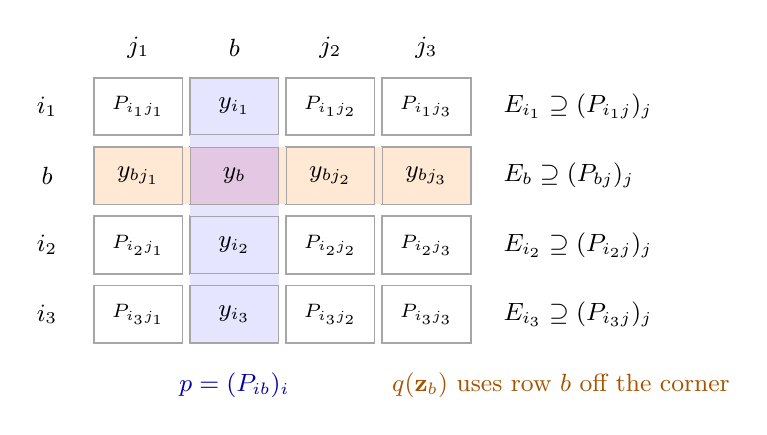
\begin{tikzpicture}[x=1.22cm,y=0.88cm,
 every node/.style={font=\small},
 cell/.style={draw=black!35,minimum width=1.13cm,minimum height=0.74cm}]
 \foreach \i in {1,2,3,4}{
   \foreach \j in {1,2,3,4}{
     \node[cell] at (\j,-\i) {};
   }
 }
 \fill[blue!10] (1.54,-4.41) rectangle (2.46,-0.59);
 \fill[orange!17] (0.54,-2.41) rectangle (4.46,-1.59);
 \fill[violet!22] (1.54,-2.41) rectangle (2.46,-1.59);
 \foreach \i in {1,2,3,4}{
   \foreach \j in {1,2,3,4}{
     \draw[black!35] (\j-0.46,-\i-0.41) rectangle
                         (\j+0.46,-\i+0.41);
   }
 }
 \node at (1,-0.15) {$j_1$};
 \node at (2,-0.15) {$b$};
 \node at (3,-0.15) {$j_2$};
 \node at (4,-0.15) {$j_3$};
 \node at (0.05,-1) {$i_1$};
 \node at (0.05,-2) {$b$};
 \node at (0.05,-3) {$i_2$};
 \node at (0.05,-4) {$i_3$};
 \node at (2,-1) {$y_{i_1}$};
 \node at (2,-2) {$y_b$};
 \node at (2,-3) {$y_{i_2}$};
 \node at (2,-4) {$y_{i_3}$};
 \node at (1,-2) {$y_{b j_1}$};
 \node at (3,-2) {$y_{b j_2}$};
 \node at (4,-2) {$y_{b j_3}$};
 \node[font=\scriptsize] at (1,-1) {$P_{i_1j_1}$};
 \node[font=\scriptsize] at (3,-1) {$P_{i_1j_2}$};
 \node[font=\scriptsize] at (4,-1) {$P_{i_1j_3}$};
 \node[font=\scriptsize] at (1,-3) {$P_{i_2j_1}$};
 \node[font=\scriptsize] at (3,-3) {$P_{i_2j_2}$};
 \node[font=\scriptsize] at (4,-3) {$P_{i_2j_3}$};
 \node[font=\scriptsize] at (1,-4) {$P_{i_3j_1}$};
 \node[font=\scriptsize] at (3,-4) {$P_{i_3j_2}$};
 \node[font=\scriptsize] at (4,-4) {$P_{i_3j_3}$};
 \node[anchor=west] at (4.7,-1) {$E_{i_1}\supseteq(P_{i_1j})_j$};
 \node[anchor=west] at (4.7,-2) {$E_b\supseteq(P_{bj})_j$};
 \node[anchor=west] at (4.7,-3) {$E_{i_2}\supseteq(P_{i_2j})_j$};
 \node[anchor=west] at (4.7,-4) {$E_{i_3}\supseteq(P_{i_3j})_j$};
 \node[blue!65!black,anchor=north] at (2,-4.7)
   {$p=(P_{ib})_i$};
 \node[orange!65!black,anchor=north] at (5.4,-4.7)
   {$q(\mathbf z_b)\text{ uses row }b\text{ off the corner}$};
\end{tikzpicture}
\caption{The square under $\lambda_Z$. Blue marks column $b$, whose
old parameter array is $p$; orange marks the row containing the added
outputs used by $q$. Their common corner has parameter $w=P_{bb}$.
The new parameters $E_i$ contain the respective old parameter rows.
The distinguished slot is drawn in second position for legibility.
The figure records marginal and factor relations, not exchangeability
of the two axes.}
\label{fig:activation-square}
\end{figure}

\begin{lemma}\label{lem:square-conditional}
In the square just defined, the conditional law of column $b$ given
$E$ is its $\lambda_Y$ law given $p$. Moreover,
\begin{equation}\label{eq:square-row-locality}
 \E_{\lambda_Z}[q(\mathbf z_b)\mid E,(y_i)_{i\in I}]
       =u(E_b,y_b).
\end{equation}
In particular, the conditional law of $y_b$ given $E$ is
$m_Y(\dd y\mid w)$; in a single $Z$-state, the conditional law of its
slot-$b$ state given $e=\omega_Z$ is the same fibre law over its old
slot-$b$ parameter.
\end{lemma}

\begin{proof}
Apply saturation of $Y$ to the extension $Z\to Y$. Under the induced
map $Z^I\to Y^I$, the old joining is precisely column $b$, and the new
datum $\mathcal D_0(Z)$ is $\sigma(E)$. Equation~\eqref{eq:saturation-identity}
for $l=0$, first on a countable determining family, gives the first
conditional-law assertion. The singleton case of
Proposition~\ref{prop:selected} then gives
\begin{equation}\label{eq:corner-fibre-law}
 \mathcal L(y_b\mid E)=m_Y(\cdot\mid w).
\end{equation}
Taking the row-$b$ marginal and applying the tower property from $E$
to its coordinate $E_b$ gives
the stated single-state assertion.

For \eqref{eq:square-row-locality}, fix $l\ne b$ and denote by
$\mathbf z_{-l}$ all rows except row $l$. Given $E$, these three rows
are independent with their $Z$ fibre laws, by
Proposition~\ref{prop:selected} applied to $Z$. In particular,
\begin{equation}\label{eq:omit-one-column-state}
 \E[q(\mathbf z_b)\mid E,(y_i)_{i\ne l}]=u(E_b,y_b).
\end{equation}
It remains to justify adding $y_l$ to the conditioning. For every
bounded measurable test $F$ of a $Y$-state, saturation for the datum
type $l$ gives
\begin{equation}\label{eq:missing-state-markov}
 \E[F(y_l)\mid E,\mathbf z_{-l}]
 =\E_{\lambda_Y}[F(y_l)\mid p,(y_i)_{i\ne l}].
\end{equation}
The right side is measurable in $(E,(y_i)_{i\ne l})$. Thus, given this
smaller datum, $y_l$ is conditionally independent of the complete rows
$\mathbf z_{-l}$. For completeness, multiplying
\eqref{eq:missing-state-markov} by any bounded function of
$\mathbf z_{-l}$ and conditioning on the smaller datum factors their
conditional product expectations. A monotone-class argument then gives
the asserted conditional independence. Since $q(\mathbf z_b)$ is
measurable in $\mathbf z_{-l}$, adjoining $y_l$ does not alter
\eqref{eq:omit-one-column-state}. This proves
\eqref{eq:square-row-locality}.
\end{proof}

We can now compute the correlation between the two highlighted lines.
First condition on the column in Lemma~\ref{lem:square-conditional},
then condition within its old law on its corner state. The result is
\begin{equation}\label{eq:square-product}
 \E\bigl[q((y_i)_i)q(\mathbf z_b)\mid E\bigr]
   =\int g(p,y)u(E_b,y)\,m_Y(\dd y\mid w).
\end{equation}
The right side is not manifestly positive. The next lemma supplies the
parameter independence that will show it cannot vanish identically.

\begin{lemma}\label{lem:parameter-reanchoring}
Under $\lambda_Z$, the variables $p$ and $E_b$ are conditionally independent
given $w=P_{bb}$.
\end{lemma}

\begin{proof}
Let $\kappa:W_Z\to W_Y$ be the factor obtained from the slot-$b$
map $Z\to Y$. This is a flow factor, and
$P_{ib}=\kappa(E_i)$. Proposition~\ref{prop:selected} identifies the
$E$ law with the ordinary deterministic-length Furstenberg law on
$W_Z$. For a bounded test $F$ of $E_b$ and a rectangle test
$\prod_i H_i(P_{ib})$, its integrated average is therefore computed
from
\[
 \int_{W_Z} F(S_{W_Z}^{bt}e)
       \prod_i H_i\bigl(\kappa(S_{W_Z}^{it}e)\bigr)\,
                         \dd m_{W_Z}(e)
\]
at each fixed $t$. Substitute $e'=S_{W_Z}^{bt}e$. The expression becomes
\[
 \int_{W_Z} F(e')
       \prod_i H_i\bigl(S_{W_Y}^{(i-b)t}\kappa(e')\bigr)\,
                         \dd m_{W_Z}(e').
\]
All factors other than $F$ depend only on $\kappa(e')$. Thus $F$ may
be replaced, at every $t$, by its conditional expectation given
$\kappa$. Averaging and taking the deterministic limit gives
\[
 \E\left[F(E_b)\prod_i H_i(P_{ib})\right]
 =\E\left[\E[F(E_b)\mid w]\prod_i H_i(P_{ib})\right].
\]
Rectangle tests generate the $p$ sigma-algebra, and $w$ is one of
its coordinates. The monotone-class theorem yields the required
conditional independence.
\end{proof}

\subsection{Nonvanishing and the additional role}

We record the elementary Hilbert-space fact used to finish the
argument. Its separability hypothesis is automatic for the probability
fibres occurring here.

\begin{lemma}\label{lem:independent-hilbert-vectors}
Let $V$ be a square-integrable random vector in a separable real
Hilbert space, and let $V'$ be an independent copy. If
$\ip V{V'}=0$ almost surely, then $V=0$ almost surely.
\end{lemma}

\begin{proof}
If $\Prob(\norm V\ge\epsilon)>0$ for some $\epsilon>0$, a countable
cover by balls of radius $\epsilon/4$ contains one ball meeting that
event with positive probability. With positive probability both $V$
and $V'$ lie in this intersection. On that event their norms are at
least $\epsilon$ and their distance at most $\epsilon/2$, so
\[
 \ip V{V'}
 =\tfrac12\bigl(\norm V^2+\norm{V'}^2-\norm{V-V'}^2\bigr)>0.
\]
This is a contradiction.
\end{proof}

\begin{proposition}\label{prop:activation}
For the saturated channel $Y$ and maximal nonzero correlation chosen
above, the regrouped channel $Z$ has a nonzero correlation
\eqref{eq:role-correlation} with output roles $A\cup\{b\}$.
\end{proposition}

\begin{proof}
We first prove that the conditional quantity in
\eqref{eq:square-product} is nonzero. In a single $Z$-state let $R(e)$
denote its old $W_Y$-parameter array; it is a function of $e=\omega_Z$.
Let $w$ denote its slot-$b$ parameter. Given $w$, write $\alpha_w$ for
the law of the old parameter array in $\lambda_Y$, and $\beta_w$ for
the law of $e$ in $m_Z$. Then $R_*\beta_w=\alpha_w$. Both old arrays,
the column array $p$ and the row array $R(E_b)$, have this same
conditional marginal. Lemma~\ref{lem:parameter-reanchoring} says that
the pair $(p,E_b)$ has conditional law $\alpha_w\otimes\beta_w$.

Work for almost every fixed $w$ in the separable real Hilbert space
$H_w=L^2(m_Y(\cdot\mid w))$. The bounded kernels
$g(p,\cdot)$ and $u(e,\cdot)$ are measurable $H_w$-valued random
vectors. To justify these assertions on a common conull set of $w$,
choose a countable generating algebra on the standard Borel space $Y$.
Its rational simple span is dense in every $H_w$; the scalar tests
against this span and Fubini give the required strong measurability.
The single-state assertion of
Lemma~\ref{lem:square-conditional} says that, conditionally on $e$,
the state $y$ has precisely the fixed law $m_Y(\cdot\mid w)$. Hence
conditioning on $R(e)$ does not introduce a $y$-dependent weight into
the distribution of $e$. The tower property for
\eqref{eq:g-and-u} gives the Hilbert-valued identity
\begin{equation}\label{eq:average-u-is-g}
 \E_{\beta_w}\bigl[u(e,\cdot)\mid R(e)\bigr]
       =g(R(e),\cdot).
\end{equation}
This can also be checked against a countable dense set in $H_w$:
the joint law of $(e,y)$ over $w$ is
$\beta_w(\dd e)m_Y(\dd y\mid w)$, and conditioning the defining
expectation of $u$ further on $(R(e),y)$ gives the defining expectation
of $g$.

Suppose now that \eqref{eq:square-product} were zero almost surely.
Conditional parameter independence would imply
\[
 \ip{g(p,\cdot)}{u(e,\cdot)}_{H_w}=0
 \quad\text{for }\alpha_w\otimes\beta_w\text{-almost every }(p,e).
\]
Average in $e$ conditionally on $R(e)$ and use
\eqref{eq:average-u-is-g}. We obtain
\[
 \ip{g(p,\cdot)}{g(p',\cdot)}_{H_w}=0
 \quad\text{for }\alpha_w\otimes\alpha_w\text{-almost every }(p,p').
\]
Lemma~\ref{lem:independent-hilbert-vectors} forces
$g(p,\cdot)=0$ almost surely for almost every $w$. This contradicts
the previously established nonvanishing of $g$.

It follows that some bounded measurable real test $\Psi(E)$ has
\begin{equation}\label{eq:activated-correlation}
 \E_{\lambda_Z}\bigl[
       \Psi(E)q((y_i)_i)q(\mathbf z_b)\bigr]\ne0.
\end{equation}
For example, take the sign of the nonzero conditional expectation
in \eqref{eq:square-product}. We identify its four roles. In every
row $i\ne b$, the factor from $q((y_i)_i)$ reads the old slot-$b$
state: when $i\in A$ it is a function of the old outputs retained in
$Z$, and when $i\notin A$ it is a function of $Z$'s original spatial
coordinate. Their spatial means remain zero. In row $b$, the factor
$q(\mathbf z_b)$ is a function of the three added lists $Q_j$.
Under the full spatial product law of the outputs of $Z$, these lists
are independent and each of its three factors is centred. Therefore
$q(\mathbf z_b)$ is itself centred for that spatial product law.
Finally $\Psi$ is a test of the full new distal parameter array $E$.
Thus \eqref{eq:activated-correlation} has exactly the form
\eqref{eq:role-correlation}, with output roles $A\cup\{b\}$, as
asserted.
\end{proof}

\begin{proof}[Proof of Theorem~\ref{thm:main}]
If the required pointwise conclusion failed, the standard coding
reduction and Proposition~\ref{prop:selectors} would supply the fixed
selectors and a nonzero correlation with no output roles. A maximal
role number $r$ would therefore exist. Proposition~\ref{prop:role-bound}
gives $r\le2$. Proposition~\ref{prop:saturation} preserves a maximal
witness in a saturated channel, and Proposition~\ref{prop:activation}
then produces a nonzero correlation with $r+1$ output roles. This
contradicts the definition of $r$. Pointwise failure is impossible.
The limiting value is the product of the four integrals, as in the
norm convergence of Lemma~\ref{lem:relative-norm}. Pulling back from
the standard coded factor proves the assertion on the original
probability space.
\end{proof}

\appendix
\section{Pointwise convergence for the proper subsets of four times}
\label{sec:lower-length}

We prove Lemma~\ref{lem:lower-length}.  The systems to which that lemma
is applied in Section~\ref{sec:selected} are extensions of a suspension
and need not be mixing or ergodic.  Accordingly, the input needed here
is a pointwise convergence theorem on arbitrary invertible probability
preserving systems.  Its analytic basis is the oscillation estimate in
\cite[Proposition~2.2]{TripleCompanion}, denoted by P in this appendix.  We also
write H for \cite{HilbertCompanion}.

P states this oscillation estimate for the times $n,2n,3n$ before using
mixing to identify its limit.  We need the three additional triples
contained in $\{1,2,3,4\}$.  We obtain them by modifying the local
four-linear construction in H and its extension to inputs varying with
depth in P.  This is a use of those analytic proofs, including their
intermediate estimates; the boundedness theorem for the trilinear
Hilbert transform alone would not supply the required oscillation
estimate.  We specify the imported statements first, then verify the
coefficient changes, and finally give the passage to arbitrary systems
and all integer averaging lengths.

\subsection{The local estimates used from H and P}

For this appendix, a \emph{role set} is a set $S$ of four distinct
integer coefficients.  Initially $S=\{0\}\cup J$, where
$J\subset\{1,2,3,4\}$ has three elements.  If $K$ is a dyadic interval
of length $r$, put
\begin{equation}
 \mathcal H_{K,S}(z)
 =r^{-2}\int_{\R^2}w_K(x,t)\prod_{j\in S}z_j(x+jt)\,\dd x\,\dd t.
 \label{eq:ll-local-form}
\end{equation}
Fix $c_0>0$ and $C_0\ge1$.  The admissible kernels are the smooth,
compactly supported functions $w_K$ for which every $x+jt$ on the
support lies in $K$ at distance at least $c_0r$ from its boundary,
\begin{equation}
 \int_{\R}w_K(v-jt,t)\,\dd t=0
 \quad(v\in\R, j\in S),
 \qquad
 \|\partial_x^a\partial_t^b w_K\|_\infty
 \le r^{-a-b}\bigl(C_0(a+b+2)\bigr)^{C_0(a+b+2)}.
 \label{eq:ll-kernels}
\end{equation}
Kernels may be chosen independently at the different intervals.

H's \emph{Uniform local estimate}
\cite[Theorem~2.2]{HilbertCompanion}
asserts, for $S=\{0,1,2,3\}$ and a suitable $q\in(2,3)$, that
\begin{equation}
 \sum_{K\in\mathcal K}|K|\,|\mathcal H_{K,S}(z)|
 \le C\int_{\R}\prod_{j\in S}M_qz_j(y)\,\dd y,
 \qquad M_qz=(M(|z|^q))^{1/q},
 \label{eq:ll-fixed-local}
\end{equation}
for every finite family of dyadic intervals and compactly supported
scalar $L^q$ inputs.  Here $M$ is the Hardy--Littlewood maximal
operator.  Its proof, in H, Sections~3--10, supplies the quantitative
chart, projection, separation, counting, and side estimates used in P.

The extension needed for oscillation is P's \emph{Local estimate with
variation in depth}, Theorem~3.2.  To state it, let $K_*$ be a root
interval and let $s(K)=\log_2(|K_*|/|K|)$ be the depth of a descendant.
For a finite integer block $B=\{a,\ldots,b\}$ and a scalar sequence
$(z_s)$, write
\[
 \mathcal V_B(z)(y)
 =\max_{s\in B}|z_s(y)|+
   \sum_{s=a}^{b-1}|z_{s+1}(y)-z_s(y)|.
\]
For the original role set $\{0,1,2,3\}$, P proves the assertion below.
We establish it for the four required role sets.

\begin{proposition}[The local analytic input with changed coefficients]
\label{prop:ll-depth}
Let $S=\{0\}\cup J$, where $J$ is a three-element subset of
$\{1,2,3,4\}$.  Let $\mathcal T$ be a finite rooted dyadic tree with
root $K_*$ and largest depth $d$, and let $\mathcal K\subset\mathcal T$
have kernels satisfying \eqref{eq:ll-kernels}.  For each $j\in S$, let
$(z_{j,s})_{0\le s\le d}$ be measurable scalar functions on $K_*$.
Extend these functions by zero outside $K_*$.
Suppose that $\{0,\ldots,d\}$ has a deterministic partition into
$W_j\ge1$ nonempty consecutive blocks, on each of which
\[
 \mathcal V_B(z_j)(y)\le W_j^{-1/2}
 \quad\text{for almost every }y\in K_*.
\]
The partitions may differ between the four roles.  Then
\begin{equation}
 \sum_{K\in\mathcal K}|K|
   \bigl|\mathcal H_{K,S}((z_{j,s(K)})_{j\in S})\bigr|
 \le C(c_0,C_0)|K_*|.
 \label{eq:ll-depth}
\end{equation}
The constant is independent of the tree, kernels, depth range, and
block partitions.  It can be chosen uniformly over the four sets $S$.
\end{proposition}

The proof of Proposition~\ref{prop:ll-depth} is the proof-by-modification
below.  The analytic inputs are H's local estimate and its proofs of the
intermediate estimates, and P's depth-local construction in Sections~4--7.
Proposition~\ref{prop:ll-depth} is the sole analytic input to the
local-to-orbit argument in Subsection~\ref{subsec:ll-transfer};
Subsection~\ref{subsec:ll-convergence} then proves
Lemma~\ref{lem:lower-length}.  The intervening subsections establish
the proposition by checking, in order, the coordinate and quadratic
identities, the integer-lift and counting arithmetic, and their
use in P's depth scheduling.
We retain their definitions of quadratic chart atoms, inherited
projection families, curvature tags, and finite progression tests.  The
following computations specify their dependence on the four role
coefficients.  In particular, the proposition is not an assertion of
uniform continuity of a Hilbert-transform bound in its slopes.

\subsection{Coordinate changes and the quadratic cancellation vector}
\label{subsec:ll-algebra}

Every set $S$ above contains an adjacent pair.  Translate all role
labels by the same integer so that one such pair is $0,1$.  This is the
change of variables $x'=x+mt$ in \eqref{eq:ll-local-form}, with
Jacobian one.  The four spatial coordinates themselves are unchanged.
Consequently the support and cancellation conditions remain the same,
and the derivative bounds retain their form after increasing the fixed
constant $C_0$.  During the local argument we use these translated
labels.  Their pairwise differences have absolute value at most four,
and their diameter is either three or four.  Thus
\begin{equation}
 |t|\le |K|/3
 \quad\text{whenever every }x+jt\text{ lies in }K.
 \label{eq:ll-support-t}
\end{equation}

The vector $(-1,3,-3,1)$ in H is replaced by a primitive integer vector
$(c_j)_{j\in S}$ proportional to
\[
 \left(\prod_{\ell\in S\setminus\{j\}}(j-\ell)\right)^{-1}.
\]
The overall sign is immaterial.  Before translation, convenient choices
are
\begin{equation}
\begin{array}{c|rrrr}
 S&\multicolumn{4}{c}{(c_j)_{j\in S}\text{ in increasing role order}}\\ \hline
 \{0,1,2,3\}&-1&3&-3&1\\
 \{0,1,2,4\}&-3&8&-6&1\\
 \{0,1,3,4\}&-1&2&-2&1\\
 \{0,2,3,4\}&-1&6&-8&3
\end{array}
\label{eq:ll-coefficient-table}
\end{equation}
Lagrange interpolation of the polynomials $1,u,u^2$ gives
\begin{equation}
 \sum_{j\in S}c_j=\sum_{j\in S}jc_j=
 \sum_{j\in S}j^2c_j=0.
 \label{eq:ll-moments}
\end{equation}
These identities are preserved by translation of the role labels.
Every $c_j$ is nonzero.  All coefficients and denominators arising
from this finite list of coordinate systems are bounded absolute
constants.

We distinguish numerical role labels from enumerations of four
objects.  A coefficient such as $j$, $j-i$, or $c_j$ is changed according
to $S$.  An ordering of four input sizes, four leaves, or four positions
in a multilinear expansion still enumerates four objects.  This
convention leaves those parts of H's proofs unchanged.

\subsection{Chart separation, detection, and the scale estimates}

The local absolute estimate, H, Lemma~2.1, uses the map
$(x,t)\mapsto(x+it,x+jt)$, whose determinant is $j-i$.  Its endpoint
bounds and interpolation therefore hold for the new roles.  In
particular the initial bound for the finite-depth constant in
\eqref{eq:ll-fixed-local}, and H's stopping reduction to normalized
local sizes, remain valid.  The coefficient and projection bounds,
compression and height-bin estimates, H, Lemmas~3.2--3.5, are
statements about finite families of vectors or real frequencies and do
not specify a progression coefficient.

We next check the part of H, Section~4, that converts two chart atoms
in distinct roles into separated factors.  A chart phase has the form
\[
 \lambda y^2+(\theta y)^TCd+\beta y,
\]
where $\theta$ is a vector of real frequencies, $C$ is the rational
chart matrix, and $d$ is a bounded lift of $\theta y$ modulo the
integer lattice.  The source definition also includes a smooth
amplitude on the lift.  Its one-variable Weyl estimates, Fourier
expansion, and uniform tail estimates are unchanged.

For H, Lemma~4.5 (\emph{Progression separation}), fix source roles $i,k$
and spectator roles $a,b$.  Set $\alpha_i=1$, $\alpha_k=0$, and solve
\[
 \sum_{j\in S}\alpha_j=\sum_{j\in S}j\alpha_j=0
\]
for $\alpha_a,\alpha_b$.  This is possible because $a\ne b$.
Writing $y_j=x+jt$, insert the same lift partitions as in H at
$\theta y_a$, $\theta y_b$, and $\theta t$.  If their lifts are
$d_a,d_b,d$, then
\[
 k_j=d_j-d_a-(j-a)d
\]
is an integer vector.  For instance, if $d_j=\theta y_j-m_j$ and
$d=\theta t-m$, the identity $y_j=y_a+(j-a)t$ gives
$k_j=-m_j+m_a+(j-a)m$.  Thus the equality cutoffs in H still test
integer carries exactly.  Their support bounds change only by a
fixed factor.  With $A_2=\sum_jj^2\alpha_j$, direct expansion gives
\begin{equation}
 \begin{split}
 \sum_{j\in S}\alpha_j
       [\lambda y_j^2+(\theta y_j)^TCd_j]
 &=A_2[\lambda t^2+(\theta t)^TCd]\\
 &\quad+\sum_{j\in S}\alpha_j(\theta y_j)^TCk_j.
 \end{split}
 \label{eq:ll-chart-identity}
\end{equation}
The last sum is linear in $x,t$ and hence separates in $y_a,y_b$.
The smooth amplitude on the bounded lift box has the same Gevrey
bounds up to fixed constants.  Fourier expansion therefore gives
H's absolutely convergent separation into two spectator atoms and one
atom in $t$, with the same coefficient-tail exponents and
quasipolynomial complexity bounds.  H, Lemma~4.6 (\emph{Single-scale separation}), then uses $t=(y_b-y_a)/(b-a)$; every added rational height is
bounded by an absolute constant.

For the generalized von Neumann bound, H, Lemma~4.11, let $i$ be
the role whose input is controlled by its $U^3$ norm.
Apply Cauchy--Schwarz in the directions $(-j,1)$ for the other
three roles, beginning with the role containing the $L^2$ input.
Each direction holds $x+jt$ fixed and changes $x+it$ by
$(i-j)h$.  Multiplication by the nonzero integer $i-j$ preserves Haar
measure on a circle.  The three independent circle parameters
therefore produce the same cube integral as in the source proof.
Character weights split using the marked pair $x=y_0$,
$t=y_1-y_0$.  Enlarging the fixed periodic boxes accommodates all
translated role sets.  This verifies the coefficient-dependent part
of the generalized von Neumann bound.  In H, Lemma~4.12
(\emph{Local detection}), the potentially unbounded $L^2$ residual
occupies a different role.  After clipping the opposing inputs, the
source proof decomposes two of them using its continuous inverse
theorem and bounds the uniform errors by Lemma~4.11.  The separated
chart moments then detect the residual.  Those separations were
verified above; the clipping, inverse theorem, and mixed-norm
exponents are unchanged.

H, Lemma~5.1 (\emph{A scale sum for one separated term}),
uses the spectator coordinates $(y_a,y_b)$.  Holding one fixed, the
integral of the kernel over the other is zero by
\eqref{eq:ll-kernels}, with a constant Jacobian factor $|b-a|$.
The double primitive of that kernel consequently has the same
compact support and smooth bounds.  Its tensor expansion into
mean-zero bumps, the Bessel estimates for those bumps, and the
frequency-height bounds apply with the new pair.  The only additional
demodulations have frequencies $\pm\gamma/(b-a)$; their rational
multipliers have bounded height, although $\gamma$ can be arbitrary
real.  This also verifies the coefficient changes
in the finite predictor list and the delayed predictor replacement.
The scale bands, accuracy gaps, and projection-energy bounds in the
remaining base construction depend on these estimates and the
four-slot multilinearity, rather than the values of the labels.
There is also a multivariable use of the chart estimates in H,
Lemma~5.7 (\emph{Few active scales for a fixed triple}).  Squaring
the transpose at the remaining role $\ell$ gives six atoms with
arguments $h+(j-\ell)t$ and $h+(j-\ell)t'$.  These are still fixed
integer linear forms in three variables, so the three-variable Weyl
alternative and chart expansion of H, Lemmas~4.3--4.4, apply with
the same complexity bounds.  Its final kernel cancellation is
the marginal at anchor $\ell$ in \eqref{eq:ll-kernels}.

\subsection{Curvature tags, short blocks, and integer heights}

H's localization in Section~6 groups chart atoms by their normalized
quadratic phase and horizontal chart data, called their curvature
tags.  Normalize the parameters $(\lambda,C)$ in role $j$ by
dividing both by $c_j$, and retain the horizontal vector $\theta$.
The coefficient calculation in H, Lemma~6.1 (\emph{Separation of different tags}), can
then be checked directly.  For source roles $i,j$ and spectator roles
$a,b$, put
\[
 \xi_\ell=\frac{b-\ell}{b-a},\qquad
 \zeta_\ell=\frac{\ell-a}{b-a};
 \qquad y_\ell=\xi_\ell y_a+\zeta_\ell y_b.
\]
The barycentric formula gives
\begin{equation}
 c_i\xi_i\zeta_i=-c_j\xi_j\zeta_j\ne0.
 \label{eq:ll-tag-identity}
\end{equation}
Indeed the factors $(i-a)(i-b)$ cancel from the product defining
$c_i$, leaving a nonzero multiple of $(i-j)^{-1}$; interchanging
$i,j$ changes its sign.  The return calculation in that lemma
therefore has the same nonzero prefactor and the same separation
conclusion.  Its period is enlarged to clear these fixed denominators.

The residue-template calculation in H, Lemma~6.6
(\emph{A uniform same-tag test}), uses the
marked adjacent pair.  Its lifts satisfy
\begin{equation}
 d_\ell=(1-\ell)d_0+\ell d_1+k_\ell,
 \qquad k_\ell\in\Z^d.
 \label{eq:ll-template-lift}
\end{equation}
Substitution of \eqref{eq:ll-template-lift} and
\eqref{eq:ll-moments} cancels the common quadratic terms and leaves
only linear phases from the carries.  Their Fourier expansion has
the same residue-template bound after a fixed enlargement of the
lift box.  It introduces no new curvature tag.  Thus the source
localization proof receives the same tag-separation and transfer
estimates.  Its graph distances, color histories, masks, and
projection bounds are then used with those estimates and their
original parameter order.

H, Lemma~7.2 (\emph{Short-block comparison}), uses two sampling
windows to compare a finite lattice form with a form on a connected
torus.  Place those windows on roles $0,1$.  The lattice and lifted
torus coordinates in the other roles are respectively
\[
 n_j=(1-j)n_0+jn_1,
 \qquad w_j=(1-j)u+jv.
\]
Both formulas have integer coefficients.  A fixed torus of length
$64$ and lift boxes in $[-12,12]$ accommodate the present role sets;
the source support parameter is decreased by a fixed factor if
necessary.  Maps from a pair of variables to two distinct role
coordinates are injective on their lattice images and surjective on
connected tori.  These are the pair-coordinate properties needed in
the comparison.

The quadratic randomization in role $j$ becomes
$e(\gamma m^2/c_j)$, where $e(v)=\exp(2\pi i v)$ and $\gamma$ is
uniform modulo a common multiple of all $|c_j|$; the value $24$ works
for \eqref{eq:ll-coefficient-table}.  On the Fourier support of the
four-linear form,
\[
 \sum_jm_j=\sum_jjm_j=0.
\]
The two vectors $c=(c_j)$ and $(jc_j)$ are independent and span this
two-dimensional nullspace.  Hence $m_j=c_j(v+jv')$ for some real
$v,v'$, and
\[
 \sum_j\frac{m_j^2}{c_j}
 =\sum_jc_j(v+jv')^2=0
\]
by \eqref{eq:ll-moments}.  The randomization preserves the form.
For each single role, averaging its fourth moment in the spatial
variable and in $\gamma$ imposes equality of a pair's sum and sum of
squares; the same two pairings as in H remain.  Thus its fourth-moment
and clipping estimates, including their powers of $q-2$, are
unchanged.

The return from lattice points to small intervals also holds with
these coordinates.  If four real role coordinates are within $e$ of
integers, the marked adjacent pair reconstructs an integer progression.
The discrepancy at any other role is an integer of magnitude less
than $8e$.  Choosing $e<1/100$ forces it to vanish.  The admissible
real offsets have positive area, computed explicitly below in
\eqref{eq:ll-polygon}.  All support and overlap losses in the
short-block comparison are therefore fixed constants.

The remaining arithmetic change is the height base.  In H,
Sections~8--9, replace $L_h=6^h$ by $L_h=12^h$, and replace the
factor $36$ in the finite progression tests by $144$.  Anchor changes
still have integer coefficients.  The common progression multiplier
in H, Section~8.3, uses exactly \eqref{eq:ll-template-lift} and
\eqref{eq:ll-moments}, so its smoothness and Fourier truncation are
unchanged in type.  For the divisibility step, a coordinate in the
free lattice quotient in H, Lemma~8.3 (\emph{Height stabilization}),
is an integral rational multiple of $12^{R'}$.  Here the quotient
is the integer coordinate lattice modulo its intersection with the
source's small rational subspace, $R'$ is the height gap, and $C_*$
bounds the denominators before multiplication by $12^{R'}$.
The intersection is saturated, so this quotient is free abelian.
Writing $\Delta$ for the required drop in height, its $2$- and $3$-adic
valuations are at least
\[
 2R'-\log_2 C_*,\qquad R'-\log_3 C_*.
\]
Thus $R'>\log_2C_*+2\Delta$ ensures divisibility by $12^\Delta$.
No assumption that the initial denominator has only primes $2,3$ is
needed: the resulting coordinate is already integral.  The reserves
and the later growth constant $A_0$, used in the source bounds
$E_h=A_0^{h+1}$, are chosen using the new base.

\subsection{Progression counting and the depth-varying extension}

We finish the coefficient check at the finite counting step because
it requires more than the identities for quadratic phases.  In H,
Section~9, eliminating a role $\ell'$ gives the three coefficients
\[
 \alpha_i=i-\ell',\qquad i\in S\setminus\{\ell'\}.
\]
They are nonzero and have absolute value at most four.  The
horizontal frequency tests use sums of role frequencies, while their
anchored tests use the weights $i-\ell'$.  Their kernel cancellations
are precisely \eqref{eq:ll-kernels}.  Accordingly the source's
Fourier expansions, coefficient tails, and annular tests keep their
forms after these replacements.

In H, Lemma~9.1 (\emph{Sparse mass of separated progression tests}),
the shift data consist of a vector $\zeta\in\R^d$ and integer
vectors $n$ with $\|n\|_\infty\le B$.  Replace the shifts
$36n\cdot\zeta$ in its annular relations by $144n\cdot\zeta$,
and the neighborhood shifts $6n\cdot\zeta$ by $12n\cdot\zeta$.
The parameter $N_0$ is the coefficient reserve for the latter
neighborhoods.  The proof uses a fine common grid; choose its step
on a multiple clearing the integers $1,2,3,4$.

For a four-step path, alternately add its four annular relations.
The intermediate label in role $i$ and the two labels in a second
role cancel, leaving $\alpha_i(a-a')$ and an expression in the
four color labels.  Dividing by $\alpha_i$ constructs the source's
difference cover.  The required lattice compatibility is
\begin{equation}
 \frac{144}{\alpha_i}\in12\Z,
 \qquad \frac{12\alpha_j}{\alpha_i}\in\Z.
 \label{eq:ll-counting-divisibility}
\end{equation}
Both assertions hold because $|\alpha_i|$ divides $12$.
The integer vector obtained by adding four original shifts has
norm at most $4B$.  In units of the new neighborhood shift $12$,
division by $\alpha_i$ therefore gives a vector of norm at most
$4B\cdot12/|\alpha_i|\le48B$.
The reserve $N_0\ge64B$ accommodates it.  The scalar error is at most
four times one relation's error after division by a nonzero integer.

For the slab cover, write the first two coordinates as their box
centers plus shifts $12n_i\cdot\zeta$ and scalar interval errors.
Substitute them in the three-role relation and solve for the third
coordinate.  The resulting shift coefficients are
$12\alpha_1/\alpha_3$, $12\alpha_2/\alpha_3$, and
$144/\alpha_3$.  By \eqref{eq:ll-counting-divisibility} they are
integers, and the resulting shift vector has norm at most
$C(d+1)^2B$ as in H.  Choose the separation reserve and
the excluded pure-shift interval constants larger by the fixed
factors arising from these substitutions.  The covering iterations
use the same orders of sumsets, the graph count uses the same four
roles, and the block and scale counts use the same covers.  Their
exponents are consequently unchanged.  In particular the source
factor $L^{29}\delta^{1/2080}$ remains valid, where $L$ bounds the
number of scale occurrences of a fixed pair of labels and $\delta$
is the sparse tuple-density threshold.  In the application, let
$\xi$ be the vector of frequencies obtained from the height
construction and take $\zeta=\xi/144$, so the available heights start at
$12^{\Delta-2}$ instead of $6^{\Delta-2}$.  The preceding height
reserves supply the required shift sizes.  Pair determination in
the application divides only by role differences, and the
short-block windows were checked above.  This verifies the
coefficient-dependent hypotheses of the counting estimate and its
application, not merely its formal conclusion.

We can now apply the remaining operator and summation arguments of
H.  The main projection families, Fourier modes, and counting tests
have the same bounds in powers of logarithms of their budgets.  The
coordinate changes have inserted only fixed rational heights,
fixed derivative losses, and the replacement of one fixed
exponential height base by another.  None changes a budget exponent
as a function of the final $q$.  H's Section~10 chooses those
exponents before taking $q\in(2,3)$ sufficiently close to two;
its absorption of the finite-depth constant therefore applies to
the modified estimates.  This proves \eqref{eq:ll-fixed-local} for
the four role sets together with the intermediate estimates used
in P.

It remains to carry these inputs through P's depth-local proof.
The \emph{Maximal estimate for local catalog rows},
\emph{The depth-varying row estimate}, and
\emph{Smooth mean-zero rows on depth inputs} in P, Section~4,
concern Hilbert-space operators supported on nested dyadic cells.
Here a catalog consists of finitely many vector-valued column
functions, each with a dyadic birth cell; descendants use restrictions
of the same functions.  A local projection is the orthogonal
projection in the cell's $L^2$ space onto constant-coefficient
combinations of a specified set of available columns.
Their hypotheses specify cellwise constant coefficients in a
persistent catalog, an ordinary fixed-input Bessel bound, and
nondecreasing input-read indices.  They contain no role coefficients.
These are P, Lemmas~4.3, 4.4, and 4.6.  The replacement just proved
supplies their same scalar and Bessel inputs.

More concretely, P, Lemma~5.3, Corollary~5.4, and Lemma~5.5,
use
$(y_a,y_b)$ and the demodulations $\pm\gamma/(b-a)$ already checked.
Their cutoff equal to one on $[-1/3,1/3]$ still covers the support
by \eqref{eq:ll-support-t}.  Separating the kernel gives exactly
mean-zero bump rows, with fixed complete carriers.  Clump replacement
and predictor rows have the same Bessel bounds because the
cancellation and height estimates have just been verified.  The
support and observation partitions of the rows, and their
nondecreasing reads of the depth inputs, are unchanged.  In P,
Section~6, use the normalized tags from \eqref{eq:ll-moments}; the
mask, template-transfer, short-block, and counting estimates are
then the versions established above.  Scheduling the column
updates and summing their row bounds introduces no new arithmetic
operation on a role label.

For completeness, the final parameter dependence can be seen in
the retained estimates of H, Section~10.3, and P, Section~7.
Write $k$ for the accuracy logarithm, $\mathfrak p$ for their
growth parameter, $K_0$ for the resulting depth-block length, and
$G_0$ for the strong energy and projection overhead.  The term
requiring $q$ close to two has the form
\[
 \mathfrak p^{-1/2}G_0(K_0+2)^{C_{19}(q-2)},\qquad
 K_0\le C_q(1+k+\mathfrak p)^{C_5},\qquad
 G_0=\exp\!\bigl(C_q(1+\log(2k))^C\bigr).
\]
Here we have renamed the source parameter $P$ to avoid confusion
with the manuscript P.  The degrees $C,C_5,C_{19}$ have absolute
bounds fixed before $q$.  The short-block estimate feeding this
term has the explicit exponent $11(q-2)/(q-1)$ in H, Lemma~7.2;
the coefficient changes above affect its fixed constants, not this
exponent.  Taking $q$ so close to two that
\[
 \max\{C_{19}^{\rm H}C_5^{\rm H},
       C_{19}^{\rm P}C_5^{\rm P}\}(q-2)<1/8
\]
is therefore permitted in both proofs.  Here the accuracy scheme
fixes $0<\theta<1$ before $q$, and the positive constant $\alpha$
is chosen sufficiently small after $q$, as in the source proofs.
Their later choice $\mathfrak p=\lceil\exp(\alpha k^\theta)\rceil$ gives
$G_0=\mathfrak p^{o(1)}$ and makes the displayed term at most
$C_q\mathfrak p^{-1/4}$.  The remaining accuracy exponents and
summations retain their source order of choice.  P's depth-local
proof consequently gives \eqref{eq:ll-depth}.

Translating the role labels back restores $S=\{0\}\cup J$.
P's depth-local theorem permits variation in any role, and the
local constructions allow any role as testing slot.  Thus this
translation does not require the testing role to remain the marked
role $0$ during the local proof.
This completes the proof of Proposition~\ref{prop:ll-depth}.

\subsection{From local forms to orbit oscillation}
\label{subsec:ll-transfer}

An \emph{averaging profile} is a real compactly supported smooth
function $\varphi$ satisfying
\begin{equation}
 \int\varphi=1,\qquad \int t^a\varphi(t)\,\dd t=0\quad(1\le a\le3),
 \qquad
 \|\varphi^{(n)}\|_\infty\le
       (G(n+2))^{G(n+2)}\quad(n\ge0)
 \label{eq:ll-profile}
\end{equation}
for some $G\ge1$.  Profiles may have either sign.  Write
$\varphi_A(t)=A^{-1}\varphi(t/A)$.  These are the profiles of P,
Section~2.

\begin{proposition}[Oscillation for the four triples]
\label{prop:ll-oscillation}
Let $(Y,\nu,R)$ be an invertible probability preserving system,
let $J\subset\{1,2,3,4\}$ have three elements, and let the functions
$g_j:Y\to\C$, $j\in J$, be measurable with $|g_j|\le1$.
For an averaging profile set
\[
 V_k^\varphi(y)=\sum_{n\in\Z}\varphi_{2^k}(n)
                   \prod_{j\in J}g_j(R^{jn}y),\qquad k\ge0.
\]
There is $C_\varphi<\infty$ such that, for all deterministic integers
$0\le k_1<\cdots<k_{W+1}$,
\begin{equation}
 \sum_{b=1}^W\int_Y
   \max_{k_b\le\ell\le k_{b+1}}
      |V_\ell^\varphi-V_{k_b}^\varphi|\,\dd\nu
 \le C_\varphi\sqrt W.
 \label{eq:ll-oscillation}
\end{equation}
The constant is independent of the system, inputs, endpoints, and $W$.
\end{proposition}

\begin{proof}
We give the transfer with the changed coefficients, following P,
Section~3.  Set $b=\varphi_2-\varphi$.  Its moments through order
three vanish, so it has a compactly supported fourth primitive $g$,
with $g^{(4)}=b$.  Choose $B\ge1$ containing its support, a smooth
Gevrey bump $u$ of integral one supported in $[-1/8,1/8]$, and a
dyadic integer $D>32B$.  For $S=\{0\}\cup J$ put
\[
 F(z,\sigma)=u(z)D^{-3}g(D\sigma),\qquad
 \mathcal W(z,\sigma)=
       \prod_{j\in S}(\partial_\sigma-j\partial_z)F(z,\sigma).
\]
The four differential operators commute.  Each is differentiation
along a line on which one role coordinate is fixed, giving all
cancellations in \eqref{eq:ll-kernels}.  On the support,
$|z+j\sigma|\le1/8+4B/D<3/8$.  Thus the rescaled kernel on an
interval of length $r=DA$ has the required interior margin.
The derivative bounds have the form \eqref{eq:ll-kernels}, with
constants depending only on the profile.  Integration in $z$ kills
every term containing a $z$ derivative, leaving
\begin{equation}
 \frac1r\int_\R\mathcal W(z,t/r)\,\dd z
 =A^{-1}b(t/A)=\varphi_{2A}(t)-\varphi_A(t).
 \label{eq:ll-kernel-normalization}
\end{equation}

Let $\Delta_k=\varphi_{2^{k+1}}-\varphi_{2^k}$ and let $f_j$,
$j\in J$, be bounded by one and supported in an interval of length
$L$.  Suppose the testing functions $f_{0,k}$ have the same support
and satisfy the block variation bound $W^{-1/2}$ over a fixed
partition of $k_-\le k\le k_+$ into $W$ blocks.  Apply
Proposition~\ref{prop:ll-depth} to dyadic cells of length $D2^k$,
then average the translated lattice over one period of its largest
scale.  All nonzero cells lie below roots of total length at most
$L+2D2^{k_+}$.  Scale order is the reverse of depth order, which
preserves block variation.  The normalized translation average
of a scale's kernels is \eqref{eq:ll-kernel-normalization}.
We obtain
\begin{equation}
 \left|\sum_{k=k_-}^{k_+}\int_{\R^2}
     f_{0,k}(x)\prod_{j\in J}f_j(x+jt)\Delta_k(t)
       \,\dd x\,\dd t\right|
 \le C_\varphi(L+D2^{k_+}).
 \label{eq:ll-continuous-test}
\end{equation}

For clarity, integer transfer does not require consecutive roles.
Plant each integer sequence on intervals of radius $e<1/200$ about
the integers.  If $x+jt$ lies in such intervals in all four roles,
use an adjacent pair to reconstruct integers $m,n$.  Every other
integer center must equal $m+jn$, since its discrepancy has
magnitude less than $8e$.  Write $x=m+\xi$, $t=n+\eta$.
The offset domain is
\[
 \Omega_{S,e}=\{(\xi,\eta):|\xi+j\eta|<e\text{ for all }j\in S\}.
\]
If $s_-=\min S$ and $s_+=\max S$, the intermediate inequalities
follow from the two extreme ones by convexity.  Hence
\begin{equation}
 |\Omega_{S,e}|=\frac{4e^2}{s_+-s_-}.
 \label{eq:ll-polygon}
\end{equation}
Replacing $\Delta_k(n+\eta)$ by $\Delta_k(n)$ has, after summing
in $n$, error $O_\varphi(2^{-k})$ per integer $m$: its derivative
is $O_\varphi(2^{-2k})$, it has $O_\varphi(2^k)$ relevant integer
arguments, and $|\eta|\le2e$.  Summing over $k\ge0$ costs
$O_\varphi(L)$.  Dividing by the fixed area
\eqref{eq:ll-polygon} therefore gives the discrete counterpart of
\eqref{eq:ll-continuous-test} with bound
$C_\varphi(L+D2^{k_+})$.

Fix a finite interval $\mathcal E$ of integer testing points
inside the common support interval of the integer sequences.
For each $m\in\mathcal E$ and block $b$, choose a maximizing
endpoint $\ell_b(m)$ and a unimodular scalar $\alpha_b(m)$ making
the selected difference nonnegative.  Set, on that scale block,
\[
f_{0,k}(m)=\frac{\alpha_b(m)}{4\sqrt W}
       \mathbf1_{\{k_b\le k<\ell_b(m)\}}.
\]
Set $f_{0,k}(m)=0$ for $m\notin\mathcal E$.
Its supremum plus variation is at most $1/(2\sqrt W)$.
The discrete test telescopes into $1/(4\sqrt W)$ times the sum
of the block maxima.  Thus its oscillation bound is
$C_\varphi\sqrt W(L+D2^{k_{W+1}})$.

We transfer the sequence inequality along finite orbit segments,
following Calder\'on's transference method \cite{Calderon}.
Apply the estimate to the finite orbit sequences
$g_j(R^r y)$ for $1-Q\le r\le M+Q$, set to zero elsewhere, where
$Q=\lceil4B_\varphi2^{k_{W+1}}\rceil$ and
$\supp\varphi\subset[-B_\varphi,B_\varphi]$.
Take $\mathcal E=\{1,\ldots,M\}$.  At these testing points all
averages are the untruncated
orbit averages evaluated at $R^m y$.  Integrate in $y$, use
invariance, divide by $M$, and let $M\to\infty$.  The result is
\eqref{eq:ll-oscillation}.  This step uses only invertibility,
measurability, and preservation of the probability measure.
\end{proof}

\subsection{Convergence on arbitrary systems}
\label{subsec:ll-convergence}

We now prove Lemma~\ref{lem:lower-length} from
Proposition~\ref{prop:ll-oscillation}.  The use of quantitative
oscillation bounds to prove pointwise convergence belongs to the
classical approach developed in \cite{JonesKaufmanRosenblattWierdl}.
The criterion needed here has the following short proof.
A uniformly bounded
sequence of measurable functions satisfying
\eqref{eq:ll-oscillation} is Cauchy almost everywhere.  Indeed, if
its tail oscillation exceeds $4\epsilon$ on a set $E$ of positive
measure, then for every fixed initial endpoint $k$ the supremum
of $|V_\ell-V_k|$ over $\ell\ge k$ exceeds $2\epsilon$ on $E$.
By monotone convergence one can choose a deterministic later endpoint
so that the corresponding integral maximum is at least
$\epsilon\nu(E)$.  Recursively choosing endpoints gives a lower
bound $W\epsilon\nu(E)$, contradicting the upper bound
$C_\varphi\sqrt W$ for large $W$.  The finite sums defining
$V_k^\varphi$ are uniformly bounded because the profile is bounded
and compactly supported.  Thus every fixed profile gives almost
everywhere convergence.

P, Lemma~2.8 (\emph{Approximation with three vanishing moments}),
states that for every $c\in[1,2]$ and every $\epsilon>0$ there is
an averaging profile with
\begin{equation}
 \|\varphi-h_c\|_1<\epsilon,
 \qquad h_c(t)=c^{-1}\mathbf1_{(0,c]}(t).
 \label{eq:ll-profile-approximation}
\end{equation}
The use of signed profiles is essential to this assertion.  One
first smooths $h_c$, preserving integral one.  The other three
moments can be canceled, without changing the integral, by four
broad translated bumps at distance and width comparable to a large
parameter $A$.  Their moment matrix for orders $0,1,2,3$, after
division of row $j$ by $A^j$, is a fixed invertible Vandermonde-type
matrix.  The prescribed zeroth correction is zero and the remaining
normalized corrections are $O(A^{-1})$.  The correcting coefficients
are therefore $O(A^{-1})$, and their total $L^1$ cost tends to zero.  The bumps
retain the derivative bounds in \eqref{eq:ll-profile} with a
profile-dependent constant.

Fix a triple $J$ and write
$a_n(y)=\prod_{j\in J}g_j(R^{jn}y)$, so $|a_n(y)|\le1$.
For $N_k=\lfloor c2^k\rfloor$, the Riemann-sum comparison gives,
uniformly in $y$,
\begin{equation}
 \limsup_{k\to\infty}
 \left|\frac1{N_k}\sum_{n=1}^{N_k}a_n(y)-V_k^\varphi(y)\right|
 \le\|h_c-\varphi\|_1.
 \label{eq:ll-profile-error}
\end{equation}
To see this, first replace $N_k^{-1}$ by $(c2^k)^{-1}$, at cost
$O(2^{-k})$, then bound the difference by
$2^{-k}\sum_{n\in\Z}|h_c(n2^{-k})-\varphi(n2^{-k})|$.
This converges to the displayed integral because the integrand is
compactly supported and piecewise continuous.

Choose countably many profiles with errors tending to zero for each
rational $c\in[1,2]$.  On their common conull set, the existence of
all the smooth-profile limits and \eqref{eq:ll-profile-error} show
that the ordinary averages along $N_k$ are Cauchy.  The
Host--Kra norm convergence theorem \cite[Theorem~1.1]{HostKra},
stated for arbitrary invertible probability preserving systems,
gives an $L^2$ limit for the averages at all integer lengths: apply
it to the four consecutive powers, inserting the constant function
one at the omitted role.  The bounded pointwise limit along each
$N_k$ must equal this $L^2$ limit almost everywhere, by bounded
convergence and uniqueness of norm limits.  Thus all rational-$c$
subsequences have the same limit on one conull set.  No identification
of that limit and no mixing assumption is needed.

Finally, for $M\le N$ and $|a_n|\le1$,
\[
 \left|\frac1N\sum_{n=1}^Na_n-\frac1M\sum_{n=1}^Ma_n\right|
 \le 2\frac{N-M}{N}.
\]
For any rational mesh of $[1,2]$, every sufficiently large integer
$N$ lies within its relative mesh size, up to $O(N^{-1})$, of some
$\lfloor c2^k\rfloor$ from that finite mesh.  Its finitely many
subsequences have the common pointwise limit.  The preceding
inequality, followed by meshes of size tending to zero, proves
convergence along all positive integers.  Homogeneity removes the
normalization $|g_j|\le1$.  A proper subset with fewer than three
roles is contained in one of the triples already treated; assign
the constant function one to its additional roles.  This proves
Lemma~\ref{lem:lower-length} in its full stated scope.

\begin{thebibliography}{99}
\raggedright

\bibitem{Assani}
I. Assani,
\emph{Multiple recurrence and almost sure convergence for weakly mixing
dynamical systems},
Israel J. Math. \textbf{103} (1998), 111--124.

\bibitem{Austin}
T. Austin,
\emph{Pleasant extensions retaining algebraic structure, I},
J. Anal. Math. \textbf{125} (2015), 1--36.
\href{https://doi.org/10.1007/s11854-015-0001-9}{doi:10.1007/s11854-015-0001-9}.

\bibitem{Birkhoff}
G.~D. Birkhoff,
\emph{Proof of the ergodic theorem},
Proc. Natl. Acad. Sci. U.S.A. \textbf{17} (1931), no.~12, 656--660.

\bibitem{Bourgain}
J. Bourgain,
\emph{Double recurrence and almost sure convergence},
J. Reine Angew. Math. \textbf{404} (1990), 140--161.

\bibitem{Calderon}
A.~P. Calder\'on,
\emph{Ergodic theory and translation-invariant operators},
Proc. Natl. Acad. Sci. U.S.A. \textbf{59} (1968), no.~2, 349--353.

\bibitem{DerrienLesigne}
J.-M. Derrien and E. Lesigne,
\emph{Un th\'eor\`eme ergodique polyn\^omial ponctuel pour les
endomorphismes exacts et les K-syst\`emes},
Ann. Inst. H. Poincar\'e Probab. Statist. \textbf{32} (1996), no.~6,
765--778.

\bibitem{Fernique}
X. Fernique,
\emph{Minorations des fonctions al\'eatoires gaussiennes},
Ann. Inst. Fourier (Grenoble) \textbf{24} (1974), no.~2, 61--66.
\href{https://doi.org/10.5802/aif.506}{doi:10.5802/aif.506}.

\bibitem{FurstenbergDisjointness}
H. Furstenberg,
\emph{Disjointness in ergodic theory, minimal sets, and a problem in
Diophantine approximation},
Math. Systems Theory \textbf{1} (1967), 1--49.

\bibitem{Furstenberg}
H. Furstenberg,
\emph{Ergodic behavior of diagonal measures and a theorem of Szemer\'edi
on arithmetic progressions},
J. Analyse Math. \textbf{31} (1977), 204--256.

\bibitem{GutmanHuangShaoYe}
Y. Gutman, W. Huang, S. Shao, and X. Ye,
\emph{Almost sure convergence of the multiple ergodic average for certain
weakly mixing systems},
Acta Math. Sin. (Engl. Ser.) \textbf{34} (2018), no.~1, 79--90.

\bibitem{HostKra}
B. Host and B. Kra,
\emph{Nonconventional ergodic averages and nilmanifolds},
Ann. of Math. (2) \textbf{161} (2005), no.~1, 397--488.

\bibitem{HuangShaoYe}
W. Huang, S. Shao, and X. Ye,
\emph{Pointwise convergence of multiple ergodic averages and strictly
ergodic models},
J. Anal. Math. \textbf{139} (2019), no.~1, 265--305;
arXiv:1406.5930.

\bibitem{Jamneshan}
A. Jamneshan,
\emph{An uncountable Furstenberg--Zimmer structure theory},
Ergodic Theory Dynam. Systems \textbf{43} (2023), no.~7, 2404--2436.
\href{https://doi.org/10.1017/etds.2022.43}{doi:10.1017/etds.2022.43}.
Corrected version: \href{https://arxiv.org/abs/2103.17167v4}{arXiv:2103.17167v4}.

\bibitem{JamneshanCorrigendum}
A. Jamneshan,
\emph{An uncountable Furstenberg--Zimmer structure theory---Corrigendum},
Ergodic Theory Dynam. Systems \textbf{46} (2026), no.~1, 211--217.
\href{https://doi.org/10.1017/etds.2025.10214}{doi:10.1017/etds.2025.10214}.

\bibitem{JonesKaufmanRosenblattWierdl}
R.~L. Jones, R. Kaufman, J.~M. Rosenblatt, and M. Wierdl,
\emph{Oscillation in ergodic theory},
Ergodic Theory Dynam. Systems \textbf{18} (1998), no.~4, 889--935.

\bibitem{KoszMirekPeluseWanWright}
D. Kosz, M. Mirek, S. Peluse, R. Wan, and J. Wright,
\emph{The multilinear circle method and a question of Bergelson},
arXiv:2411.09478v4, September 2, 2026.

\bibitem{KrauseMirekTao}
B. Krause, M. Mirek, and T. Tao,
\emph{Pointwise ergodic theorems for non-conventional bilinear polynomial
averages},
Ann. of Math. (2) \textbf{195} (2022), no.~3, 997--1109.

\bibitem{Kuca}
B. Kuca,
\emph{Joint ergodicity---40 years on},
arXiv:2603.18974v1, March 19, 2026.

\bibitem{Lesigne}
E. Lesigne,
\emph{Th\'eor\`emes ergodiques ponctuels pour des mesures diagonales.
Cas des syst\`emes distaux},
Ann. Inst. H. Poincar\'e Probab. Statist. \textbf{23} (1987), no.~4,
593--612.

\bibitem{HilbertCompanion}
OpenAI,
\emph{An $L^3$ bound for the trilinear Hilbert transform},
OpenAI Math Release preprint
\href{https://github.com/openai/math/blob/main/preprints/An-L3-bound-for-the-trilinear-Hilbert-transform-October-5-2026/paper.pdf}{OAI:An-L3-bound-for-the-trilinear-Hilbert-transform-October-5-2026},
2026.

\bibitem{TripleCompanion}
OpenAI,
\emph{Pointwise convergence of triple ergodic averages for mixing
transformations},
OpenAI Math Release preprint
\href{https://github.com/openai/math/blob/main/preprints/Pointwise-convergence-of-triple-ergodic-averages-for-mixing-transformations-October-4-2026/pointwise-triple-ergodic-averages-mixing-transformations.pdf}{OAI:Pointwise-convergence-of-triple-ergodic-averages-for-mixing-transformations-October-4-2026},
2026.

\bibitem{MixingCompanion}
OpenAI,
\emph{Rokhlin's multiple-mixing problem for one transformation},
OpenAI Math Release preprint
\href{https://github.com/openai/math/blob/main/preprints/Rokhlins-multiple-mixing-problem-for-one-transformation-September-23-2026/paper.pdf}{OAI:Rokhlins-multiple-mixing-problem-for-one-transformation-September-23-2026},
2026.

\bibitem{Sudakov}
V. N. Sudakov,
\emph{Gaussian random processes and measures of solid angles in Hilbert space},
Dokl. Akad. Nauk SSSR \textbf{197} (1971), no.~1, 43--45 (Russian).

\bibitem{Tropp}
J. A. Tropp,
\emph{Second-order matrix concentration inequalities},
Appl. Comput. Harmon. Anal. \textbf{44} (2018), no.~3, 700--736.
\href{https://doi.org/10.1016/j.acha.2016.07.005}{doi:10.1016/j.acha.2016.07.005}.

\bibitem{Ziegler}
T. Ziegler,
\emph{Universal characteristic factors and Furstenberg averages},
J. Amer. Math. Soc. \textbf{20} (2007), no.~1, 53--97.

\bibitem{Zimmer}
R. J. Zimmer,
\emph{Extensions of ergodic group actions},
Illinois J. Math. \textbf{20} (1976), no.~3, 373--409.
\href{https://doi.org/10.1215/ijm/1256049780}{doi:10.1215/ijm/1256049780}.

\end{thebibliography}

\end{document}
